\documentclass[a4]{article}
\usepackage{xcolor}
% \definecolor{mycolor}{RGB}{0, 102, 204}
% \renewcommand\thesection{\textcolor{mycolor}{\arabic{section}}}
% Standard margins for SLU is 3.5 cm on each side. Add this code if desired:
\usepackage[a4paper, left=3.0cm,right=2.5cm]{geometry}
\usepackage{fancyhdr}
% \usepackage[hidelinks]{hyperref}
\usepackage[
    colorlinks=true,
    linkcolor=black,
    urlcolor=blue,
    citecolor=black,
    filecolor=black,
    pdfborder={0 0 0}
]{hyperref}
\pagestyle{fancy}
\fancyhf{} 
% Definir encabezado (Header)
% \fancyhead[L]{}  % Texto a la izquierda del encabezado
\fancyhf{} % clear all header and footer fields
\fancyhead[C]{Estudio Hidrológico del Rio Paucartambo - C.H. Yuncan} % Texto centrado en el encabezado
\fancyhead[R]{Engie Energía Perú}  % Número de página a la derecha
\fancyfoot[C]{\thepage} % center bottom page number
% Necessary packages
\usepackage{tikz}
\usetikzlibrary{calc}
\usepackage{graphicx}
\usepackage{newtxtext}
\usepackage{float}
\usepackage{comment}
\usepackage{longtable}  % For acronyms
\usepackage{nomencl}    % For nomenclature
\usepackage{setspace} 

% Define nomenclature
\usepackage[utf8]{inputenc} %You can ommit it since 2018
\usepackage[T1]{fontenc}
\usepackage[T1]{fontenc}
\usepackage[english]{babel} 
\makenomenclature
\usepackage{etoolbox}
\usepackage{mathptmx}
\usepackage{fancyhdr}
\usepackage{amsmath,amsfonts,amssymb} 
\usepackage{caption} 
\usepackage{setspace}
\usepackage{graphicx} 
\usepackage{csquotes}
\usepackage{changepage}
\usepackage{subcaption}	% Para subfiguras
\usepackage{makeidx}
\usepackage{multirow}
\usepackage{array} 
\usepackage{float}
\usepackage{pdflscape} % Página horizontal
\usepackage{lscape} % Hoja horizontal
\usepackage{pdfpages}
\usepackage{wallpaper}
\usepackage{acronym}
\usepackage{tikz}% Para desarrollar funciones
\usepackage{url} % Para insertar url sin problemas
\usepackage{color} % Para texto con diferente colores
\usepackage{rotating}
\usepackage{tablefootnote} 
\usepackage{lipsum}
\usepackage{enumitem}
\usepackage[backend=biber,style=apa,citestyle = apa, sorting = nyt]{biblatex}
\usepackage{booktabs}
\usepackage{geometry}
\usepackage{caption}
\usepackage{siunitx}
\usepackage{booktabs}
\usepackage{pdflscape}
\usepackage{graphicx}
\usepackage{pdflscape}

\usepackage{textcomp}

\usepackage{siunitx}
\sisetup{
  detect-weight = true,
  detect-family = true,
  input-symbols = (),
  table-align-text-pre = false
}

\addbibresource{References/References.bib}
% Identation
\captionsetup[table]{labelfont=bf,textfont=bf,skip=6pt}
% This command changes the font style where SLU promotes Arial
\newenvironment{myfont}{\fontfamily{phv}\selectfont}{\par}
\begin{document}
\pagestyle{fancy}
% Title page
% To add this template to the main.tex file, just add the command "% To add this template to the main.tex file, just add the command "% To add this template to the main.tex file, just add the command "\include{titlePageSLU} after "\begin{docuemnt}" in the main.tex file


% In this segment, enter the desired data to be shown at the title page
\newcommand{\thesisAuthor}{CH. YUNCÁN}
\newcommand{\thesisTitle}{Estudio Hidrológico del Sistema Hídrico de la Cuenca del Rio Paucartambo}
\newcommand{\thesisSubTitle}{Central Hidroeléctrica Yuncán}
\newcommand{\thesisTitleTranslated}{Informe Técnico 2026}
\newcommand{\thesisDegree}{Engie Energía Perú}
\newcommand{\university}{Av. República de Panamá 3490}
\newcommand{\credits}{San Isidro, Lima}
\newcommand{\thesisPlaceDate}{Lima, 2026}

%------------------------------------------------------------------------------
\begin{titlepage}
\thispagestyle{empty}
\myfont
\setlength{\parskip}{0pt}

% Use this line of code if both SLU loggo and company/other institution loggo is desired. The positions are possible to change with the \hspace and \vspace syntax.
\begin{figure} [H]
\vspace{-3cm}
\centering
    \begin{minipage}[t]{.45\linewidth}
    \vspace{-0.3cm}
    \hspace*{1cm}
\includegraphics[width =1.5\textwidth]{engie_logo2.jpg} \hspace*{-1cm}
    \end{minipage}
\end{figure}

% If only the logo for SLU is desired, delete "\begin{comment}" and "\end{comment}" to use this line of code:
\begin{comment}
\begin{figure}
\vspace{-3cm}
    \hspace*{-2cm}
\includegraphics[width = 0.3\textwidth]{slu_logo_webb.png}\hspace*{-2cm}
\end{figure}
\end{comment}


% Adds background picture. Delete code if no background picture is wanted.
\begin{tikzpicture}[overlay, remember picture]
\node[anchor=south west, 
      xshift=-0.2cm, 
      yshift=-0.2cm] 
     at (current page.south west)
     {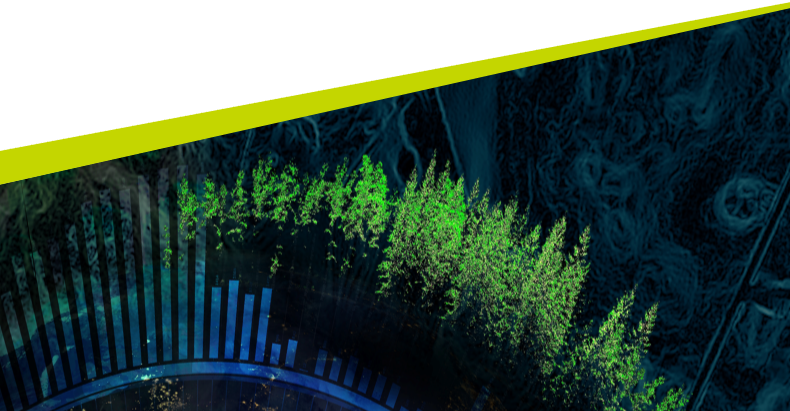
\includegraphics[width = 1.8\textwidth, height = 9cm]{background.png}}; 
\end{tikzpicture}


\vspace{1cm}
\par
\noindent
\Huge
{\raggedright
\hyphenpenalty=10000
\exhyphenpenalty=10000
\textbf{\thesisTitle}\par}
\vspace{0.2cm}
\LARGE
\par
\noindent
\\
\thesisSubTitle\\
\rule[0.3cm]{\linewidth}{2pt}
\Large

% Delete this line if no translation is desired
\noindent
\thesisTitleTranslated

\vspace{2cm}
\noindent
\LARGE
\thesisAuthor\\

\vspace{1cm}
\noindent
\large
\textbf{Elaborado por:} Carlos Enciso Ojeda\\
\noindent
\textbf{Revisado por:} Julio Loayza Daga\\

\vspace{0.5cm}
\small
\noindent
\begin{minipage}{\linewidth}
\raggedright
\thesisDegree $\cdot$ \credits\\
\university\\
\thesisPlaceDate
\end{minipage}

\end{titlepage}
 after "\begin{docuemnt}" in the main.tex file


% In this segment, enter the desired data to be shown at the title page
\newcommand{\thesisAuthor}{CH. YUNCÁN}
\newcommand{\thesisTitle}{Estudio Hidrológico del Sistema Hídrico de la Cuenca del Rio Paucartambo}
\newcommand{\thesisSubTitle}{Central Hidroeléctrica Yuncán}
\newcommand{\thesisTitleTranslated}{Informe Técnico 2026}
\newcommand{\thesisDegree}{Engie Energía Perú}
\newcommand{\university}{Av. República de Panamá 3490}
\newcommand{\credits}{San Isidro, Lima}
\newcommand{\thesisPlaceDate}{Lima, 2026}

%------------------------------------------------------------------------------
\begin{titlepage}
\thispagestyle{empty}
\myfont
\setlength{\parskip}{0pt}

% Use this line of code if both SLU loggo and company/other institution loggo is desired. The positions are possible to change with the \hspace and \vspace syntax.
\begin{figure} [H]
\vspace{-3cm}
\centering
    \begin{minipage}[t]{.45\linewidth}
    \vspace{-0.3cm}
    \hspace*{1cm}
\includegraphics[width =1.5\textwidth]{engie_logo2.jpg} \hspace*{-1cm}
    \end{minipage}
\end{figure}

% If only the logo for SLU is desired, delete "\begin{comment}" and "\end{comment}" to use this line of code:
\begin{comment}
\begin{figure}
\vspace{-3cm}
    \hspace*{-2cm}
\includegraphics[width = 0.3\textwidth]{slu_logo_webb.png}\hspace*{-2cm}
\end{figure}
\end{comment}


% Adds background picture. Delete code if no background picture is wanted.
\begin{tikzpicture}[overlay, remember picture]
\node[anchor=south west, 
      xshift=-0.2cm, 
      yshift=-0.2cm] 
     at (current page.south west)
     {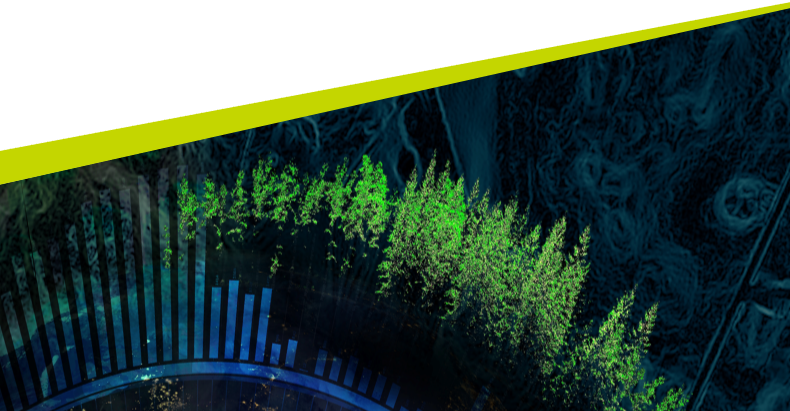
\includegraphics[width = 1.8\textwidth, height = 9cm]{background.png}}; 
\end{tikzpicture}


\vspace{1cm}
\par
\noindent
\Huge
{\raggedright
\hyphenpenalty=10000
\exhyphenpenalty=10000
\textbf{\thesisTitle}\par}
\vspace{0.2cm}
\LARGE
\par
\noindent
\\
\thesisSubTitle\\
\rule[0.3cm]{\linewidth}{2pt}
\Large

% Delete this line if no translation is desired
\noindent
\thesisTitleTranslated

\vspace{2cm}
\noindent
\LARGE
\thesisAuthor\\

\vspace{1cm}
\noindent
\large
\textbf{Elaborado por:} Carlos Enciso Ojeda\\
\noindent
\textbf{Revisado por:} Julio Loayza Daga\\

\vspace{0.5cm}
\small
\noindent
\begin{minipage}{\linewidth}
\raggedright
\thesisDegree $\cdot$ \credits\\
\university\\
\thesisPlaceDate
\end{minipage}

\end{titlepage}
 after "\begin{docuemnt}" in the main.tex file


% In this segment, enter the desired data to be shown at the title page
\newcommand{\thesisAuthor}{CH. YUNCÁN}
\newcommand{\thesisTitle}{Estudio Hidrológico del Sistema Hídrico de la Cuenca del Rio Paucartambo}
\newcommand{\thesisSubTitle}{Central Hidroeléctrica Yuncán}
\newcommand{\thesisTitleTranslated}{Informe Técnico 2026}
\newcommand{\thesisDegree}{Engie Energía Perú}
\newcommand{\university}{Av. República de Panamá 3490}
\newcommand{\credits}{San Isidro, Lima}
\newcommand{\thesisPlaceDate}{Lima, 2026}

%------------------------------------------------------------------------------
\begin{titlepage}
\thispagestyle{empty}
\myfont
\setlength{\parskip}{0pt}

% Use this line of code if both SLU loggo and company/other institution loggo is desired. The positions are possible to change with the \hspace and \vspace syntax.
\begin{figure} [H]
\vspace{-3cm}
\centering
    \begin{minipage}[t]{.45\linewidth}
    \vspace{-0.3cm}
    \hspace*{1cm}
\includegraphics[width =1.5\textwidth]{engie_logo2.jpg} \hspace*{-1cm}
    \end{minipage}
\end{figure}

% If only the logo for SLU is desired, delete "\begin{comment}" and "\end{comment}" to use this line of code:
\begin{comment}
\begin{figure}
\vspace{-3cm}
    \hspace*{-2cm}
\includegraphics[width = 0.3\textwidth]{slu_logo_webb.png}\hspace*{-2cm}
\end{figure}
\end{comment}


% Adds background picture. Delete code if no background picture is wanted.
\begin{tikzpicture}[overlay, remember picture]
\node[anchor=south west, 
      xshift=-0.2cm, 
      yshift=-0.2cm] 
     at (current page.south west)
     {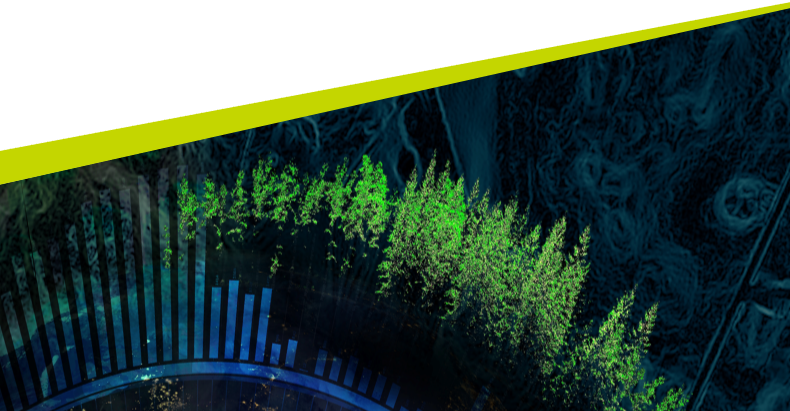
\includegraphics[width = 1.8\textwidth, height = 9cm]{background.png}}; 
\end{tikzpicture}


\vspace{1cm}
\par
\noindent
\Huge
{\raggedright
\hyphenpenalty=10000
\exhyphenpenalty=10000
\textbf{\thesisTitle}\par}
\vspace{0.2cm}
\LARGE
\par
\noindent
\\
\thesisSubTitle\\
\rule[0.3cm]{\linewidth}{2pt}
\Large

% Delete this line if no translation is desired
\noindent
\thesisTitleTranslated

\vspace{2cm}
\noindent
\LARGE
\thesisAuthor\\

\vspace{1cm}
\noindent
\large
\textbf{Elaborado por:} Carlos Enciso Ojeda\\
\noindent
\textbf{Revisado por:} Julio Loayza Daga\\

\vspace{0.5cm}
\small
\noindent
\begin{minipage}{\linewidth}
\raggedright
\thesisDegree $\cdot$ \credits\\
\university\\
\thesisPlaceDate
\end{minipage}

\end{titlepage}

% Include nomenclature
\clearpage
\onehalfspacing
\renewcommand{\nomname}{Nomenclatura}

\nomenclature{ANA}{Autoridad Nacional del Agua}
\nomenclature{BIAS}{Proporciona información sobre la tendencia del modelo a sobrestimar o subestimar una variable, nos cuantifica el error sistemático del modelo}
\nomenclature{D.E.D}{Desviación estándar de los desvíos}
\nomenclature{ENSO}{El Niño Southern Oscillation (Oscilación del sur El Niño)}
\nomenclature{HYDRACCESS}{Software hidrológico capaz de almacenar y trabajar información hidrológica en una base de datos en formato Microsoft Access 2000}
\nomenclature{IOS}{Southern Oscillation Index (Índice de Oscilación Sur)}
\nomenclature{JAXA}{Agencia de Exploración Aeroespacial Japonesa}
\nomenclature{MINAGRI}{Ministerio de Agricultura y Riego}
\nomenclature{MODIS}{Moderate Resolution Imaging Spectroradiometer (Espectroradiómetro de imágenes de moderada resolución)}
\nomenclature{MVR}{Vector Regional de Índices Pluviométricos}
\nomenclature{NASA}{National Aeronautics and Space Administration (Administración Nacional de la Aeronáutica y del Espacio)}
\nomenclature{NSE}{Índice de eficiencia de Nash-Sutcliffe}
\nomenclature{ONERN}{Oficina Nacional de Evaluación de Recursos Naturales}
\nomenclature{PET}{Potential Evapotranspiration (Evapotranspiración potencial)}

\nomenclature{R}{Coeficiente de correlación}
\nomenclature{R$^2$}{Coeficiente de determinación}
\nomenclature{RSR}{Desviación estándar de los datos medidos}

\nomenclature{SENAMHI}{Servicio Nacional de Meteorología e Hidrología del Perú}
\nomenclature{SWAT}{Soil and Water Assessment Tool (Herramienta para asesoramiento hídrico y de suelo)}
\nomenclature{TRMM}{Tropical Rainfall Measuring Mission (Misión de medida de lluvia tropical)}
\nomenclature{UH}{Unidad hidrográfica}
\nomenclature{USDA}{United States Department of Agriculture (Departamento de Agricultura de los Estados Unidos)}

\clearpage
\pagestyle{empty}
\renewcommand{\thepage}{}
\printnomenclature[1in]
\clearpage

% Table of Contents
\clearpage
\tableofcontents
\clearpage
\pagestyle{fancy}
% Include Introduction
\newpage
\section{PRESENTACIÓN}
% \section{\textcolor{mycolor}{PRESENTACIÓN}}
El propósito del presente informe es presentar al Comité de Operación Económica del Sistema Interconectado Nacional (COES-SINAC) el Estudio Hidrológico del Sistema Hídrico de ENGIE Energía Perú para el periodo 1965-2025, cumpliendo con lo estipulado en la Resolución OSINERGMIN No 196-2016-OS/CD del 02 de agosto del 2016, procedimiento técnico No 41. El Sistema Hídrico en estudio abarca la cuenca del río Paucartambo que es aprovechada con fines hidroeléctricos en la central hidroeléctrica de Yuncán - ENGIE Energía Perú S.A.\\

En la sección \ref{section:Methodology} se presenta la metodología seguida para el cálculo de caudales naturales, estimación de la precipitación satelital y su validación con las estaciones existentes en campo, identificación del número de estaciones virtuales (del satélite) de precipitación para la correcta caracterización por subcuencas y los análisis de las precipitaciones y de las series de caudales naturalizados. La sección 5 muestra la caracterización hidrológica de la cuenca del río Paucartambo hasta el embalse Yuncán (Mapa 5-1). La sección 6 presenta el modelo hidrológico distribuido \textbf{VIC (Variable Infiltration Capacity)}, sus insumos de entrada y los resultados de las simulaciones para obtener los caudales promedio mensuales desde 1998 al 2025 en los puntos QN-908 - Uchuhuerta, QN-909 – Huallamayo, QN-910 – Victoria, QN-901 + QN-902 + QN-911, y QN-903 + QN-904 + QN-905. Las salidas del modelo fueron corregidas mediante redes neuronales para ajustar los caudales simulados a los datos observados disponibles. La sección 7 muestra las discusiones y conclusiones.\\

El diagrama topológico se presenta en Mapa 4-1 junto con el mapa de la cuenca y la ubicación de las estaciones de precipitación existentes en la cuenca.\\

Se hace hincapié en los caudales mensuales naturalizados (Gráfico 6-1) y los mensuales promedios multianuales (Gráfico 6-2) en QN-908 – Uchuhuerta, los respectivos (Gráfico 6-3 y 6-4) en QN-909 – Huallamayo y para (Gráfico 6-5 y 6-6) QN-910 – Victoria I.

% Ya que la actual metodología (hidrología física) y los desarrollos tecnológicos (tecnología satelital - https://pmm.nasa.gov/GPM) permiten obtener caudales naturales directamente. No se han calculado los cambios en los embalses ni otra información adicional, ya que no se requiere. Con las metodologías antiguas, la estimación de caudales se derivaba en base a la información de los cambios en los embalses. En la actualidad, esto ya no es necesario.

\section{ANTECEDENTES}

El \textbf{COES-SINAC}, por ley, debe al \textbf{OSINERGMIN} los estudios económicos, información técnica, entre otra información necesaria para que ésta determine los precios en barra de potencia y energía del sistema interconectado. Para el cálculo de costos marginales del sistema interconectado, el \textbf{OSINERGMIN} necesita la información hidrológica de las cuencas que aprovechan las empresas generadoras.

\section{OBJETIVOS}
Los objetivos del presente documento son:
\begin{itemize}
    \item Actualizar las series de caudales naturalizados de la cuenca del río Paucartambo para el periodo 1965--2025, junto con su metodología de cálculo.
    \item Presentar las series de caudales naturalizados de la cuenca.
    \item Determinar el rango de tiempo de desplazamiento del agua desde Huallamayo hasta la central, según caudal descargado y época del año.
\end{itemize}

\section{METODOLOGÍA}\label{section:Methodology}

La Figura~\ref{fig:1a} ilustra la estructura metodológica del estudio
hidrológico. La hidrología aplicada es de tipo físico-distribuida y tiene dos
componentes principales: (1) los datos de entrada meteorológicos (precipitación,
temperatura y velocidad del viento), obtenidos a partir de productos satelitales
y de reanálisis, y (2) la caracterización del medio físico (topografía, suelos y
vegetación), que constituyen los insumos para el modelo hidrológico distribuido VIC (Variable Infiltration Capacity) \parencite{liang1994simple}. El
modelo VIC genera los caudales promedio en los puntos indicados de la cuenca
Paucartambo, desde el QN-901 hasta el QN-911. Como etapa complementaria, las
salidas del modelo fueron corregidas mediante ajuste por desviación de sesgo
(\textit{bias correction}), con el fin de ajustar los caudales simulados a los
datos observados disponibles en la cuenca.

\begin{figure}[H]
\centering
\begin{tikzpicture}[ every node/.style={font=\small}, inp/.style={rectangle,
    draw=black!65, fill=gray!30, rounded corners=2pt, minimum width=2.8cm,
    minimum height=0.65cm, text centered, inner sep=3pt, align=center},
    proc/.style={rectangle, draw=black!70, fill=gray!10, rounded corners=2pt,
    minimum width=6.5cm, minimum height=0.65cm, text centered, inner sep=3pt,
    align=center}, model/.style={rectangle, draw=black!85, fill=gray!45, rounded
    corners=3pt, minimum width=6.5cm, minimum height=0.78cm, text centered,
    font=\small\bfseries, inner sep=4pt, align=center},
    resbox/.style={rectangle, draw=black!75, fill=gray!20, rounded corners=2pt,
    minimum width=6.5cm, minimum height=0.65cm, text centered, inner sep=3pt,
    align=center}, arr/.style={-Stealth, thick, black!60} ]
% Fila 1: tres fuentes de datos
\node[inp] (chirps)  at (-3.5,  0)   {CHIRPS\\Precipitación}; \node[inp] (era5)
at ( 0,    0)   {ERA5-Land\\Meteorología}; \node[inp] (spatial) at ( 3.5,  0)
{DEM / Suelos\\Vegetación};
% Fila 2: preprocesamiento y configuración
\node[proc] (prep) at (0, -1.8) {Corrección de sesgo y configuración del
dominio}; \draw[arr] (chirps.south)  -- ++(0,-0.3) -| (prep.north west);
\draw[arr] (era5.south)    --             (prep.north); \draw[arr]
(spatial.south) -- ++(0,-0.3) -| (prep.north east);
% Fila 3: modelo VIC con spin-up indicado dentro del cuadro
\node[model] (vic) at (0, -3.2) {Modelo VIC (balance hídrico distribuido)\\
     {\small\normalfont\itshape spin-up: 4 años}}; \draw[arr] (prep) -- (vic);
% Fila 4: routing
\node[proc] (routing) at (0, -4.7) {Routing hidrológico
    (mm\,$\to$\,m\textsuperscript{3}/s)}; \draw[arr] (vic) -- (routing);
% Fila 5: corrección por sesgo
\node[proc] (bias) at (0, -5.9) {Corrección por sesgo\\
    (\textit{bias correction})}; \draw[arr]
(routing) -- (bias);
% Fila 6: salida
\node[resbox] (qnat) at (0, -7.1) {Caudales naturalizados mensuales\\
     QN-908 / QN-909 / QN-910 / QN-901,911 / QN-903,905}; \draw[arr] (bias) --
(qnat);
\end{tikzpicture}
\caption{Esquema metodológico para la estimación de caudales promedio mensuales naturales utilizando información satelital, reanálisis climático y corrección por sesgo.}
\captionsetup{labelfont=rm,skip=2pt,textfont=rm,font=small}
\label{fig:1a}
\end{figure}

Para este estudio se ha utilizado el producto
\href{https://data.chc.ucsb.edu/products/CHIRPS-2.0/}{CHIRPS Daily (Climate
Hazards Group InfraRed Precipitation with Station Data)} versión 2.0
\parencite{funk2015chirps}, en reemplazo del satélite TRMM empleado en estudios
anteriores. CHIRPS es un conjunto de datos de precipitación de alta resolución
espacial (0.05° x 0.05°, equivalente a ~5 km) y frecuencia diaria, que combina
observaciones satelitales infrarrojas con datos de estaciones meteorológicas in
situ. Esta combinación permite generar estimaciones más precisas en regiones con
topografía compleja, como la vertiente oriental de los Andes peruanos.

El producto está disponible desde 1981 hasta la actualidad, lo que lo convierte
en una fuente confiable para análisis hidrológicos de largo plazo. Su validación
con estaciones meteorológicas locales permite evaluar su desempeño en la región
de estudio. Debido a su resolución espacial, frecuencia temporal y cobertura
histórica, CHIRPS resulta particularmente adecuado para estudios de modelación
hidrológica que requieren un monitoreo detallado de la precipitación
espacio-temporal.

Por otro lado, para obtener los datos meteorológicos diarios requeridos para la
modelación hidrológica, se ha utilizado el conjunto de datos ERA5-Land Daily
\parencite{munoz2021era5land} desarrollado por el Centro Europeo de Pronósticos
Meteorológicos de Mediano Plazo (ECMWF), disponible a través de la plataforma
Google Earth Engine. ERA5-Land proporciona variables atmosféricas a alta
resolución espacial (aproximadamente 9 km) y cobertura global continua desde
1981 hasta la actualidad. Para el presente estudio, se han extraído y procesado
las variables necesarias para forzar el modelo hidrológico VIC,
incluyendo temperatura del aire a 2 metros, humedad relativa, radiación solar
superficial y velocidad del viento. Dado su enfoque orientado a aplicaciones de
superficie terrestre, ERA5-Land representa una mejora significativa respecto a
reanálisis anteriores, ofreciendo mayor resolución espacial y temporal, así como
un mejor balance de energía y agua, aspectos fundamentales para la correcta
simulación de procesos hidrológicos a escala de cuenca.

\subsection{PRECIPITACIÓN}

\subsubsection{Análisis Exploratorio de la Precipitación Regional}

La información satelital proveniente del producto
\href{https://data.chc.ucsb.edu/products/CHIRPS-2.0/}{CHIRPS Daily} fue validada
con registros pluviométricos disponibles en el área de estudio. Para ello, se
utilizó un conjunto de 17 estaciones meteorológicas con información
relativamente completa desde 1965, cuyas coordenadas y altitudes se detallan en
la Tabla~\ref{tab01}. Entre ellas, destacan las estaciones Oxapampa y San Rafael, las cuales
pertenecen a la red del SENAMHI y fueron identificadas como las únicas
disponibles dentro del dominio regional para la comparación directa con
CHIRPS.

De acuerdo con la
\href{https://www.senamhi.gob.pe/load/file/01404SENA-4.pdf}{Zonificación
Climática del SENAMHI} \parencite{senamhi2015}, el área del proyecto se
encuentra influenciada por tres zonas climáticas distintas. La parte alta
corresponde a la zona B(i) D' H3, caracterizada por un clima semifrígido y
lluvioso, con déficit de precipitaciones en invierno y humedad relativa
clasificada como húmeda. La zona media se ubica dentro del dominio B(o,i) C' H3,
con un clima frío y lluvioso, y deficiencia de lluvias en otoño e invierno.
Finalmente, la parte baja de la cuenca se encuentra en la zona A(r) B'2 H3,
donde predomina un clima templado muy lluvioso, con precipitaciones constantes a
lo largo del año y humedad relativa también considerada húmeda.

\begin{table}[ht]
\centering
\caption{Estaciones Pluviométricas Operadas por el SENAMHI/Statkraft}
\label{tab01}
\begin{tabular}{l l S[table-format=3.4] S[table-format=3.4] S[table-format=4.0]}
\toprule
\textbf{ID} & \textbf{Estación} & \textbf{Latitud (°)} & \textbf{Longitud (°)} &
\textbf{Altitud (m.s.n.m)} \\
\midrule
    01 & Altos Machay     & -10.5514 & -75.8833 & 4140 \\
    02 & Chalhuacocha     & -10.5889 & -75.8597 & 4050 \\
    03 & Hacienda Huanca  & -10.6792 & -76.0833 & 4150 \\
    04 & Huachón          & -10.6306 & -75.9472 & 3400 \\
    05 & Huallamayo       & -10.7597 & -75.7153 & 2440 \\
    06 & Huangush Alto    & -10.5722 & -75.8236 & 3885 \\
    07 & Huangush Bajo    & -10.5833 & -75.8069 & 3600 \\
    08 & Jaico            & -10.5556 & -75.9125 & 4230 \\
    09 & Victoria II      & -10.8583 & -75.9222 & 4000 \\
    10 & Lechecocha       & -10.5264 & -75.9000 & 4220 \\
    11 & Luxopata         & -10.8417 & -75.8583 & 4000 \\
    12 & Machavado        & -10.5806 & -75.8972 & 3850 \\
    13 & Manto            & -10.7403 & -75.5847 & 1870 \\
    14 & Pacchapata       & -10.5444 & -75.8958 & 4360 \\
    15 & Paucartambo      & -10.7667 & -75.8111 & 3000 \\
    16 & Puagmaray        & -10.6417 & -75.7797 & 2450 \\
    17 & Yuncán           & -10.7167 & -75.6500 & 1870 \\
    18 & Oxapampa         & -10.5926 & -76.3897 & 1825 \\
    19 & San Rafael       & -10.3217 & -76.1694 & 3053 \\
\bottomrule
\end{tabular}
\end{table}

\begin{figure}[H]
    \centering
    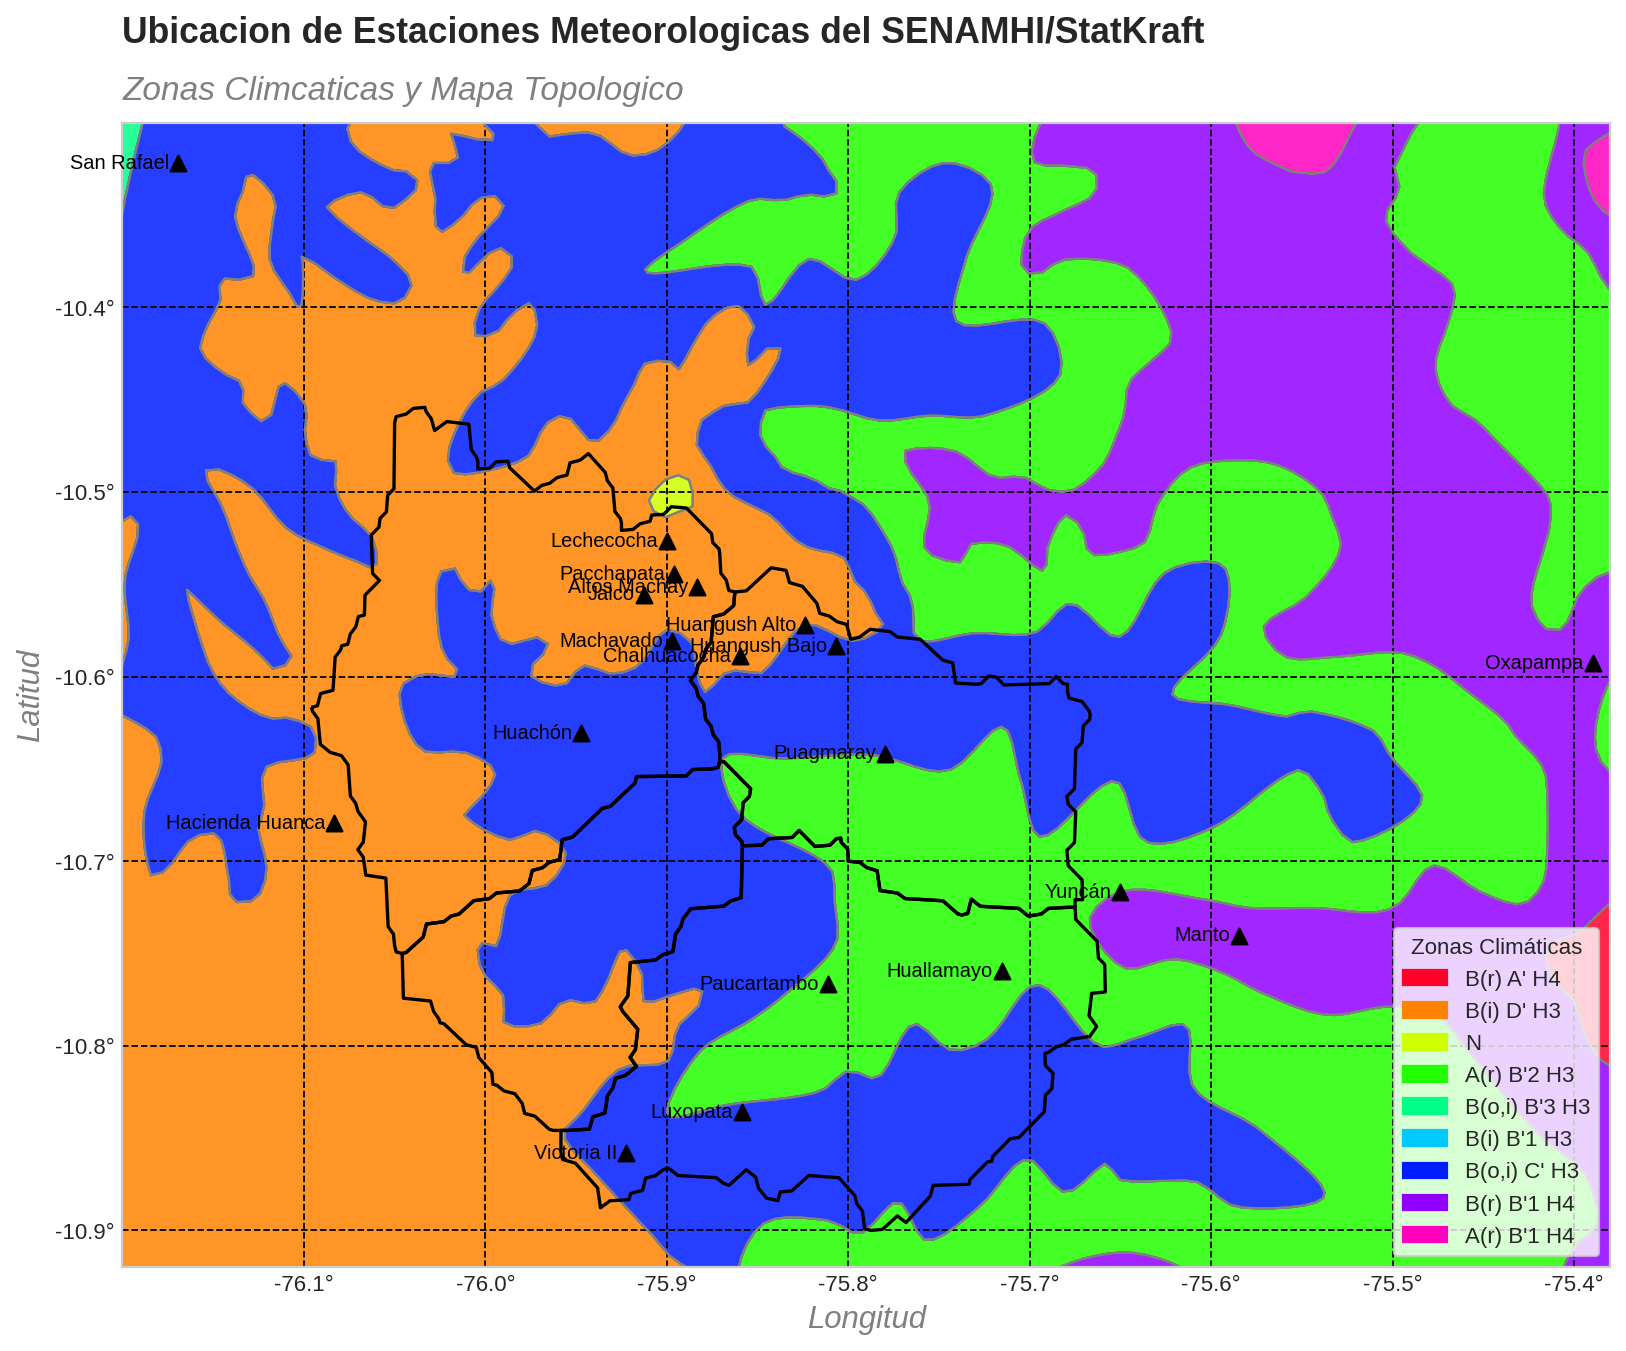
\includegraphics[width=.80\textwidth]{Figures/fig02.png}
    \caption{Ubicación de Estaciones Meteorológicas del SENAMHI/Statkraft, Zonas Climáticas y Mapas Topológico}
    \captionsetup{labelfont=rm,skip=2pt,textfont=rm,font=small}
    \label{fig:2a}
\end{figure}

\begin{figure}[H]
    \centering
    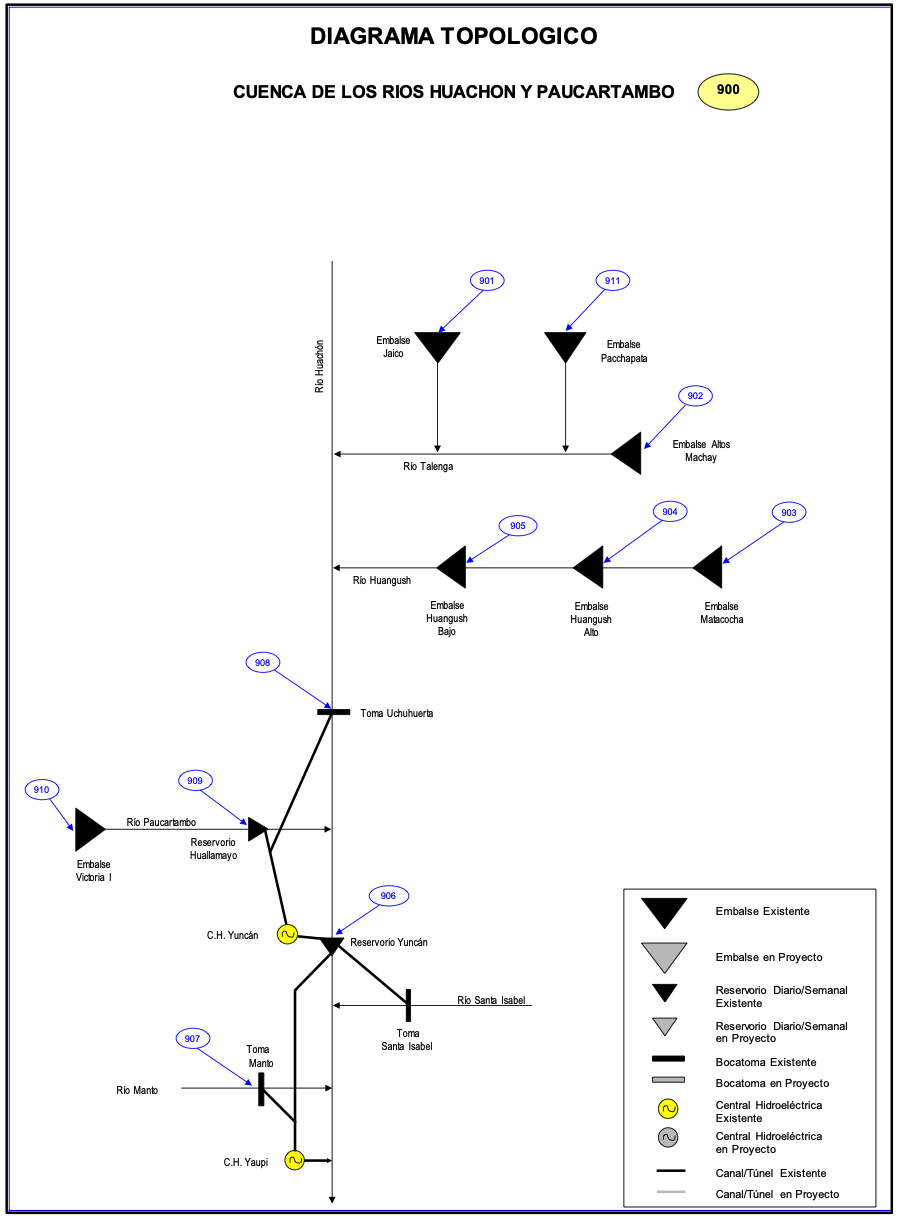
\includegraphics[width=.90\textwidth]{Figures/fig03.png}
    \caption{Diagrama Topológico. Cuenca de los Ríos Huachón y Paucartambo}
    \captionsetup{labelfont=rm,skip=2pt,textfont=rm,font=small}
    \label{fig:3a}
\end{figure}
\clearpage

Se utilizaron registros provenientes de estaciones meteorológicas locales, los
datos de precipitación histórica fueron incluidos en el Anexo 1 ("01
Precipitación Yaupi 2025.xls"), los caudales promedio mensuales del año 2025 en
el Anexo 2 ("02 QN.Paucartambo 2025.xls"), y los volúmenes de embalses en el
Anexo 3 ("03 Volúmenes 2025.xls").

\subsubsection{Validación de precipitación satelital CHIRPS}

Como parte del balance hídrico, en el presente estudio se emplearon datos
diarios de precipitación provenientes del producto satelital
\href{https://data.chc.ucsb.edu/products/CHIRPS-2.0/}{CHIRPS Daily (Climate
Hazards Group InfraRed Precipitation with Station Data)}, el cual combina
observaciones satelitales con información de estaciones terrestres para ofrecer
estimaciones de precipitación con una resolución espacial de aproximadamente 5
km y cobertura temporal desde 1981 hasta la actualidad. Para este análisis, se
consideró el período comprendido entre el 1 de enero de 1998 y el 31 de
diciembre de 2025.

Si bien se consideró inicialmente una metodología de re-escalamiento espacial
para aumentar la resolución de los productos satelitales, en el presente estudio
se optó por una estrategia distinta, aprovechando directamente la resolución
nativa del producto CHIRPS, que ofrece una malla espacial de aproximadamente 5
km. Esto permitió generar una representación de la estacionalidad espacial de la
precipitación a través de la construcción de 50 estaciones virtuales
distribuidas en el área de estudio.

Como parte del proceso de mejora de la calidad de los datos, se propuso aplicar
una corrección de sesgo (bias correction) mediante técnicas de ajuste por
cuantiles (quantile mapping) \parencite{maraun2013bias}, utilizando como
referencia las series temporales de estaciones meteorológicas terrestres
disponibles para el periodo 1998–2025. Esta metodología permitió establecer
funciones de corrección entre las distribuciones de los datos satelitales y
observados en puntos específicos, las cuales fueron empleadas para mejorar la
representatividad local de los datos de CHIRPS. De esta manera, se mejora la
representatividad de las estimaciones satelitales y se facilita la imputación de
datos faltantes en estaciones con registros incompletos.

La validación de los datos satelitales se realizó contrastando los valores
mensuales de precipitación estimados por CHIRPS con los registros observados en
estaciones meteorológicas del SENAMHI/Statkrafts, en el periodo en que ambas
fuentes se superponen (enero de 1998 a diciembre de 2025). Para este análisis se
extrajeron las series temporales de CHIRPS en las ubicaciones correspondientes a
las estaciones físicas, y se aplicaron técnicas de corrección de sesgo mediante
ajuste por cuantiles (quantile mapping) con el fin de mejorar la
representatividad local de los datos satelitales. La validación del desempeño
del producto corregido se llevó a cabo mediante métricas estadísticas
ampliamente utilizadas en estudios hidrológicos: el coeficiente de eficiencia de
Nash-Sutcliffe (NSE) \parencite{nash1970river}, el porcentaje de sesgo (BIAS),
el índice RSR (relación entre la raíz del error cuadrático medio y la desviación
estándar observada), el coeficiente de correlación de Pearson (r), el
coeficiente de determinación (R$^2$) y el índice de concordancia de Willmott (d)
\parencite{willmott1981validation}.
\newpage

\begin{figure}[H]
    \centering
    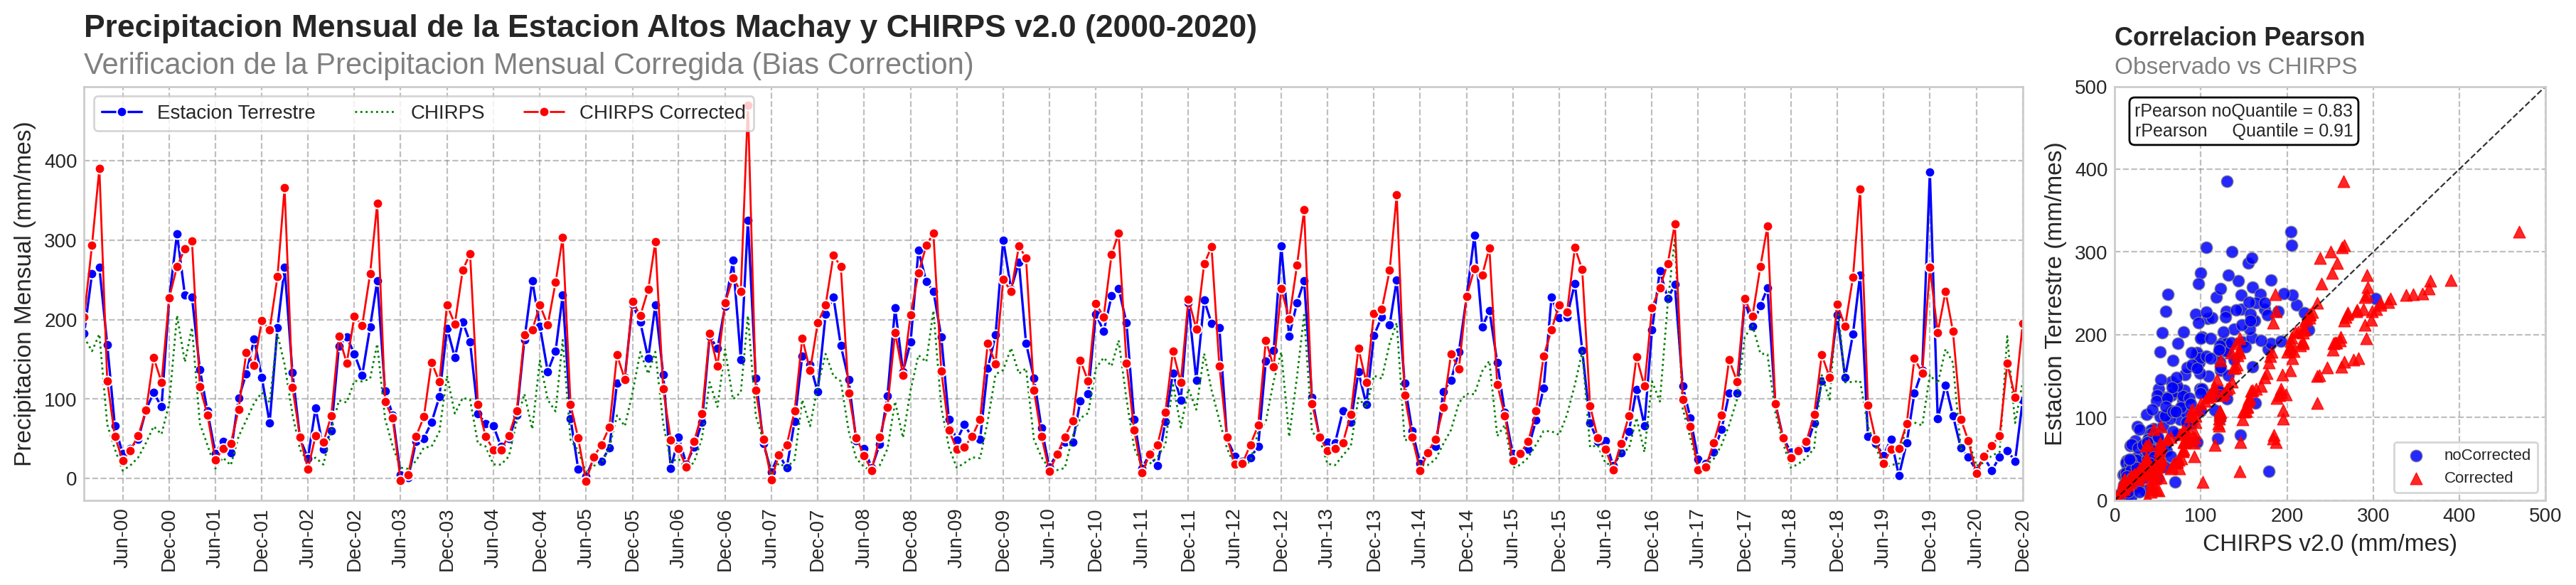
\includegraphics[angle=90, width=.31\textwidth]{Figures/fig04-1.png}
    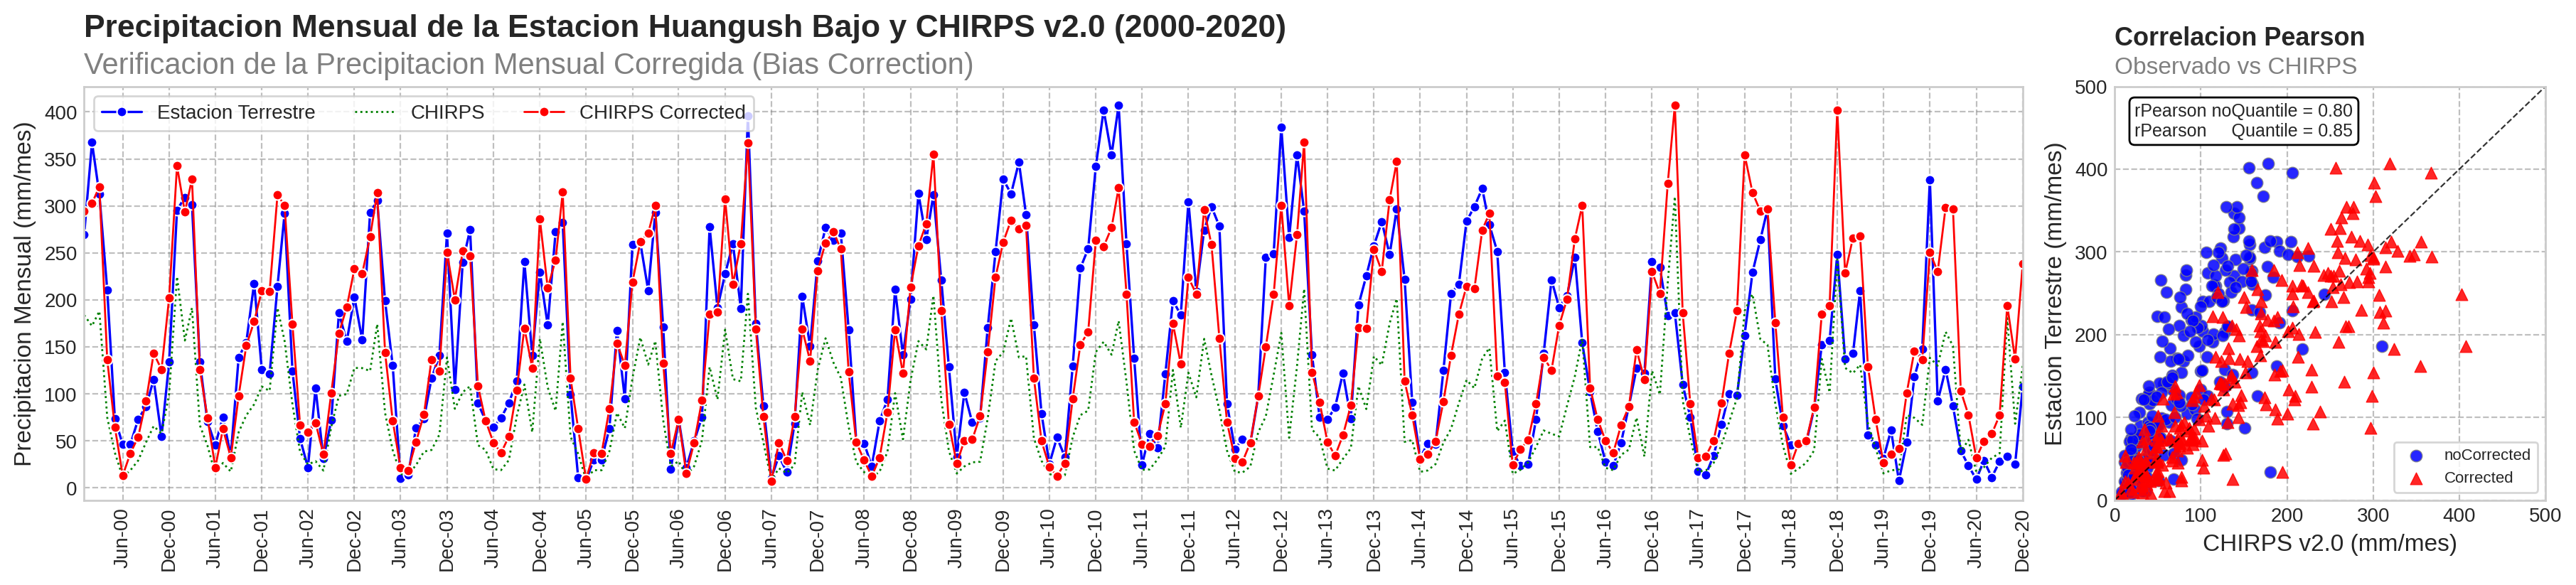
\includegraphics[angle=90, width=.31\textwidth]{Figures/fig04-2.png}
    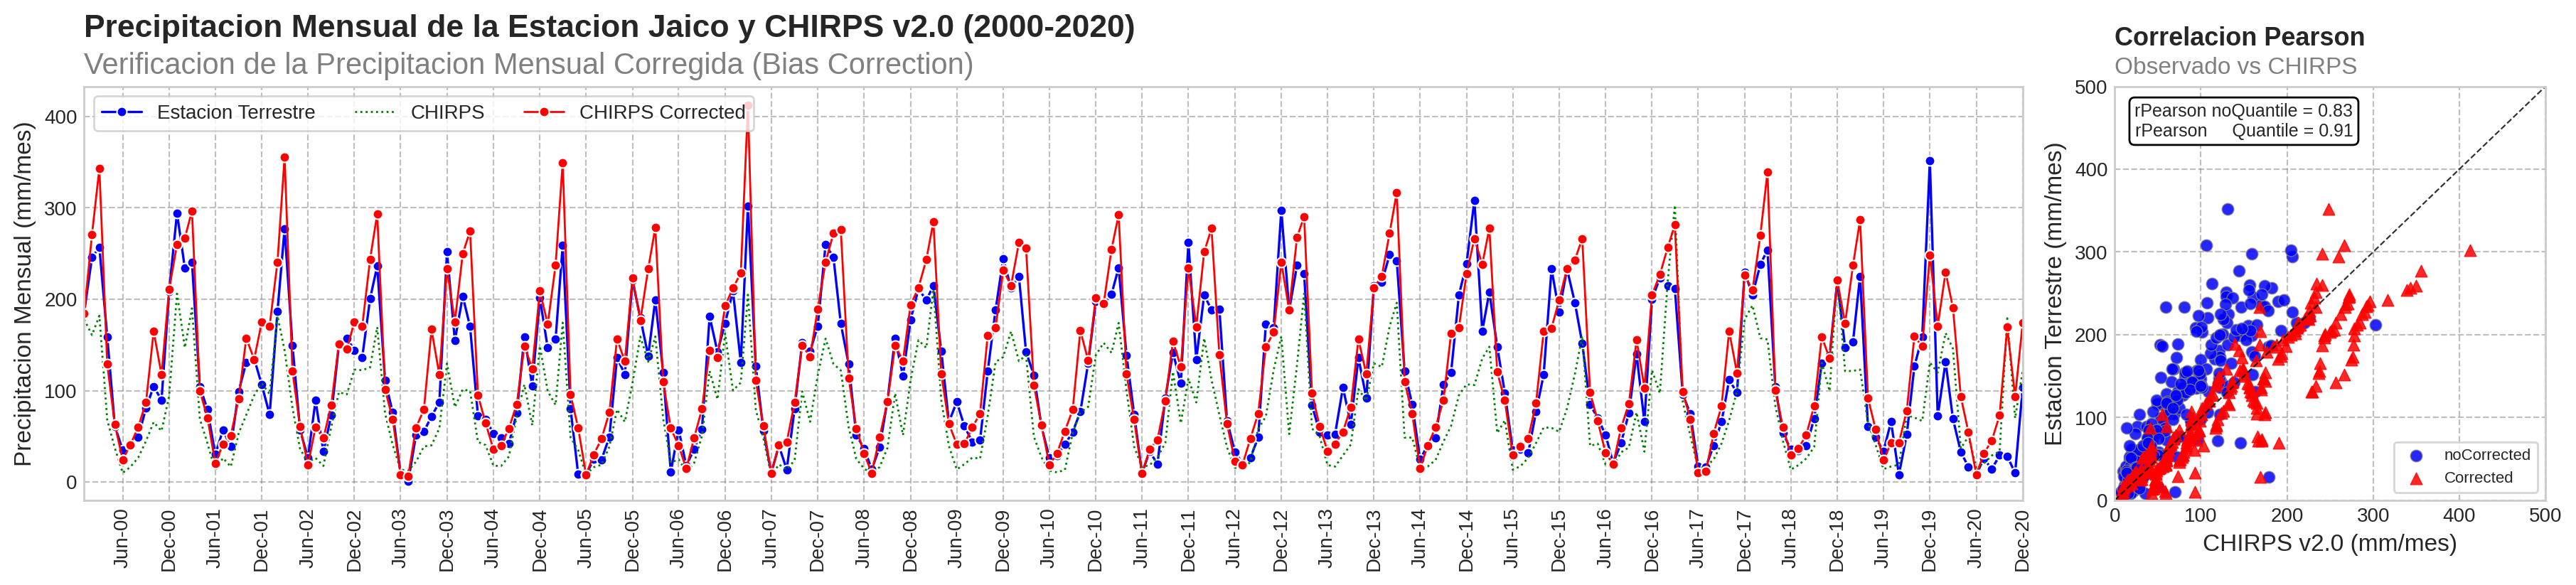
\includegraphics[angle=90, width=.31\textwidth]{Figures/fig04-3.png}
    \captionsetup{labelfont=rm,skip=2pt,textfont=rm,font=small}
    \label{fig:chirps_validacion_1}
\end{figure}
\newpage
\begin{figure}[H]
    \centering
    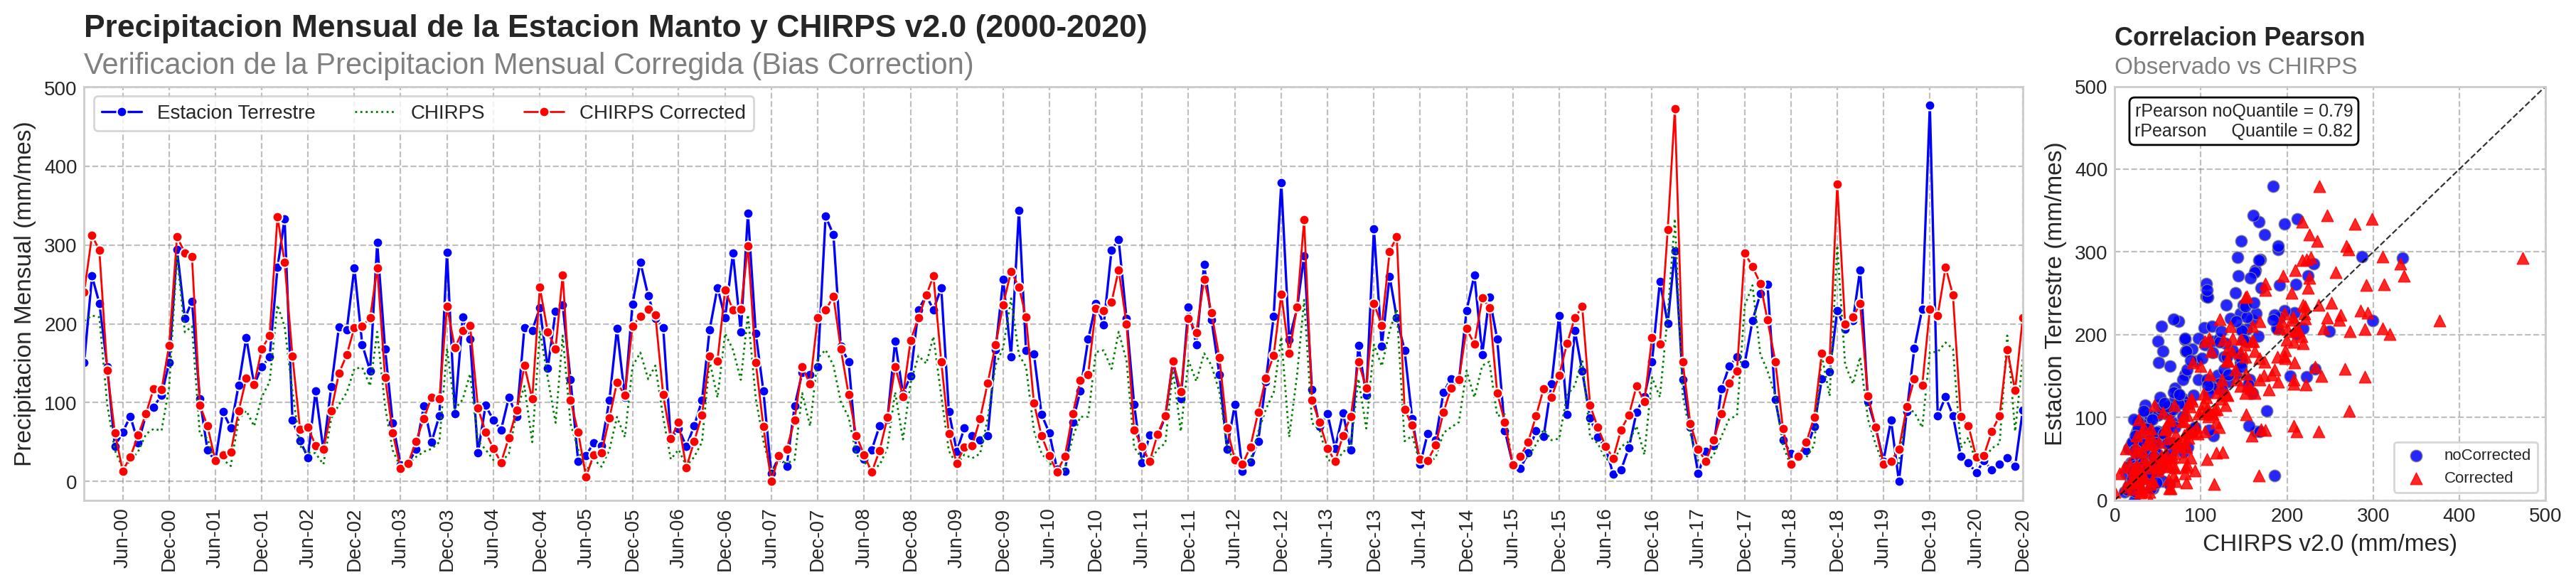
\includegraphics[angle=90, width=.31\textwidth]{Figures/fig04-4.png}
    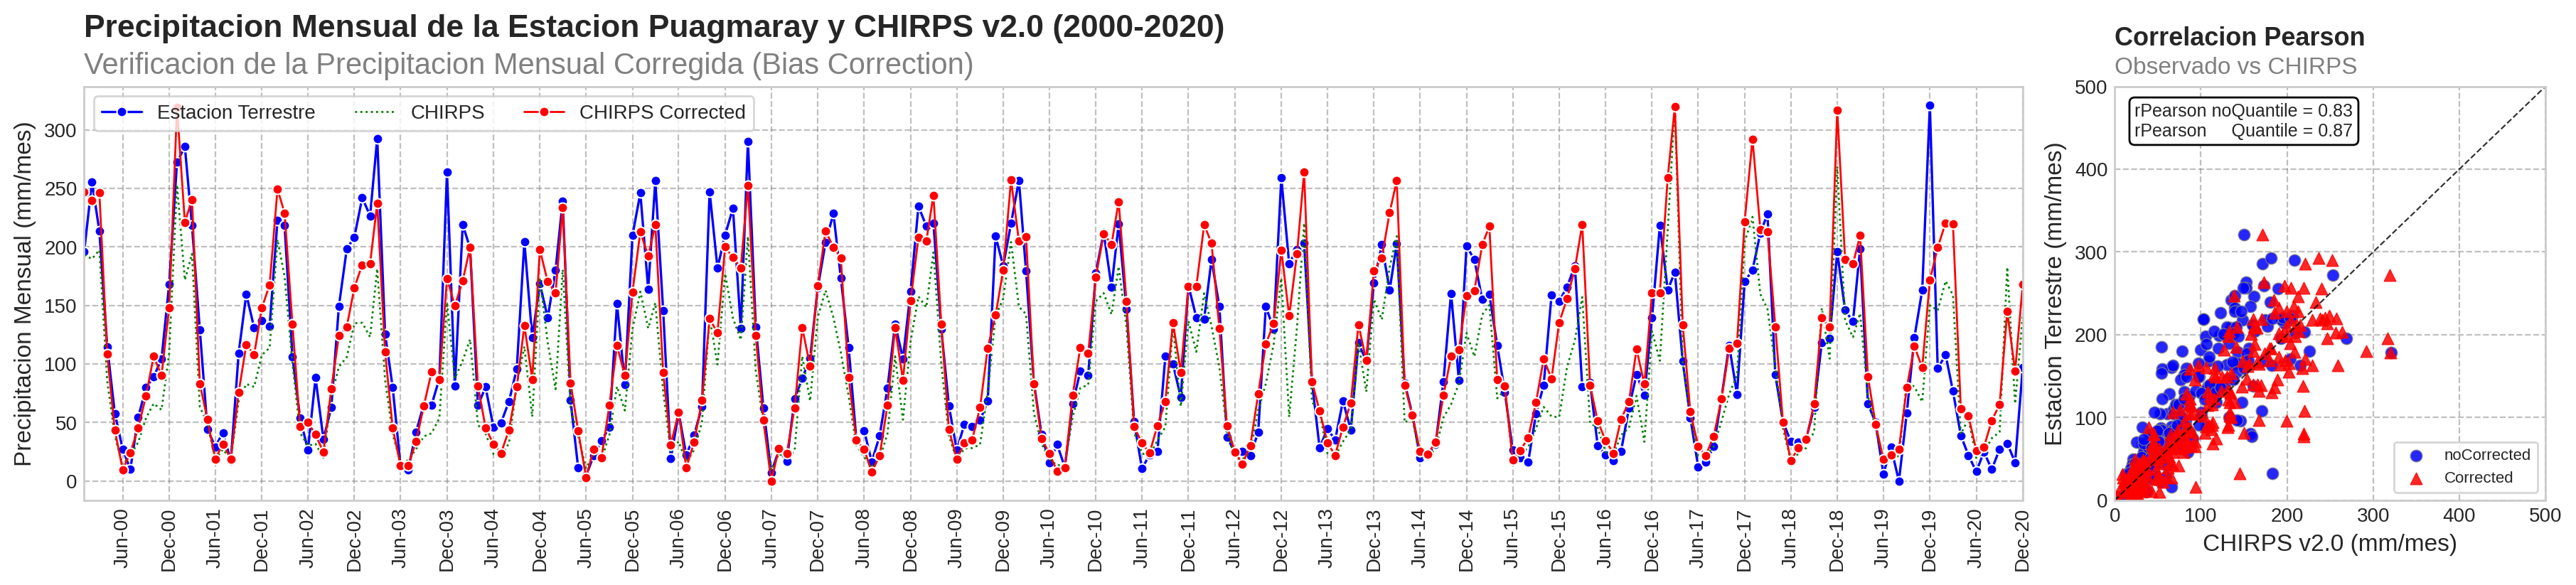
\includegraphics[angle=90, width=.31\textwidth]{Figures/fig04-5.png}
    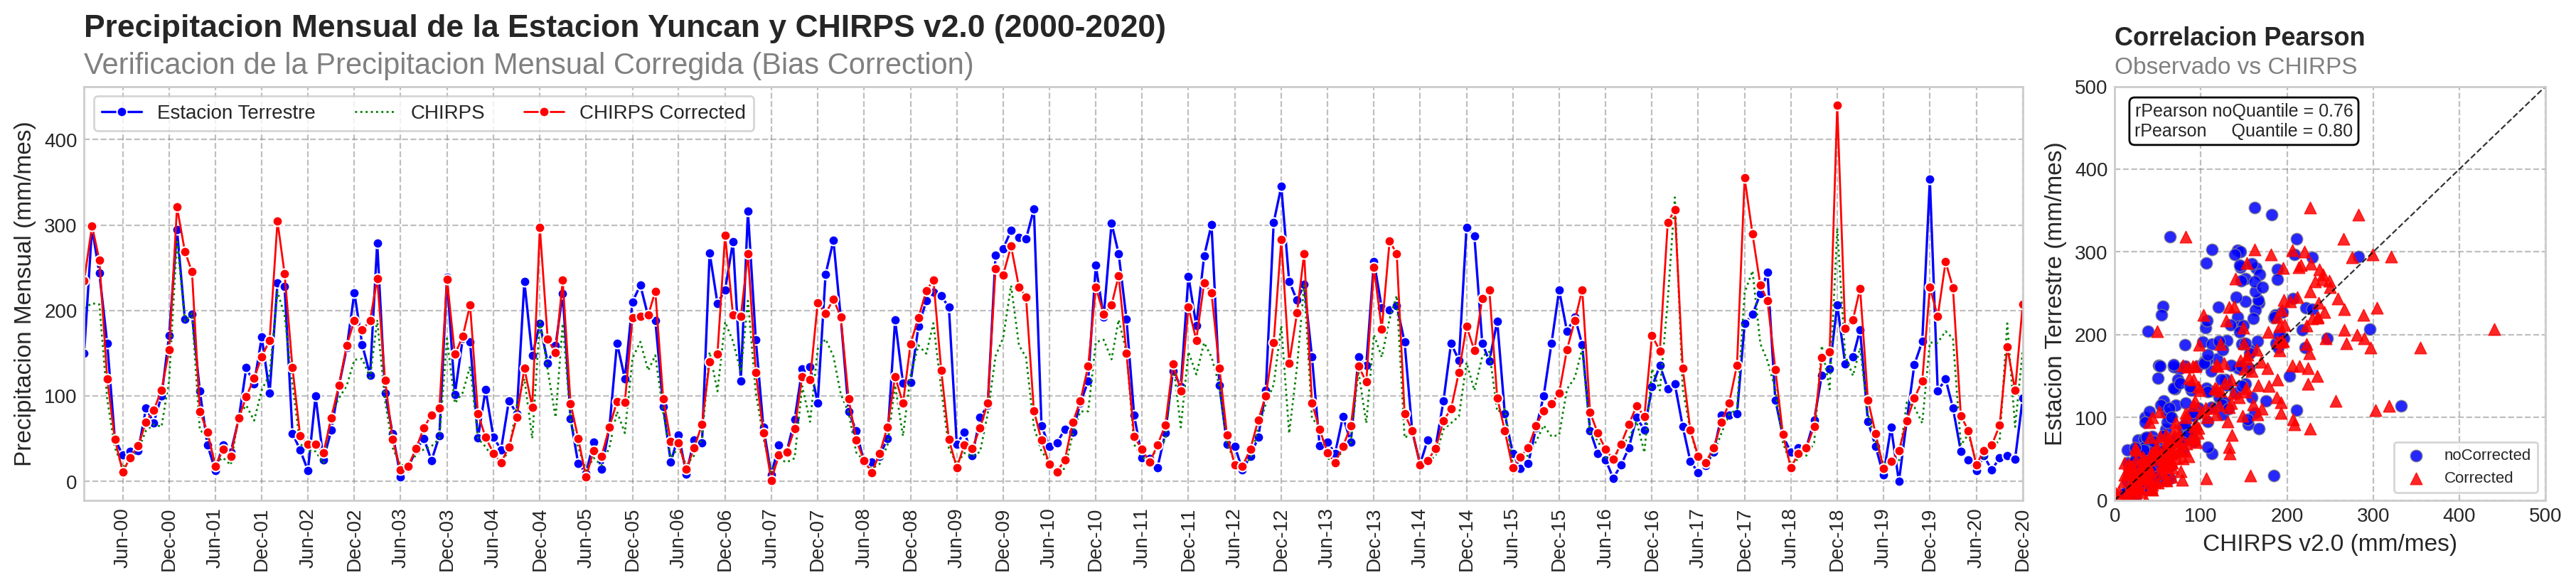
\includegraphics[angle=90, width=.31\textwidth]{Figures/fig04-6.png}
    \captionsetup{labelfont=rm,skip=2pt,textfont=rm,font=small}
    \label{fig:chirps_validacion_2}
\end{figure}
\newpage

Los resultados de los índices estadísticos calculados se presentan en las Tablas
\ref{tab02} y \ref{tab03}. De acuerdo con los análisis realizados y los
criterios de clasificación de la Tabla \ref{tab04}, se observa que las series
temporales comparadas muestran una alta similitud y correspondencia entre sí en
todas las estaciones evaluadas.

\begin{table}[ht]
\centering
\caption{Evaluaci\'on estad\'istica de las series de precipitaci\'on reconstruidas (Parte 1).}
\label{tab:reconstruccion_parte1}
\scriptsize
\begin{tabular}{l c c c c c c c}
\toprule
\textbf{Indicador} & Altos Machay & Chalhuacocha & Hacienda Huanca & Huachón &
Huallamayo & Jaico & Lechecocha \\
\midrule
NSE        & 0.73 & 0.67 & 0.64 & 0.54 & 0.51 & 0.75 & 0.73 \\
RSR        & 0.52 & 0.57 & 0.60 & 0.68 & 0.70 & 0.51 & 0.52 \\
PBIAS      & 5.51 & 2.72 & 9.72 & 8.60 & 8.31 & 3.95 & 0.84 \\
RMSE       & 42.59 & 50.46 & 32.53 & 33.72 & 50.49 & 39.44 & 42.35 \\
r          & 0.87 & 0.84 & 0.84 & 0.80 & 0.77 & 0.88 & 0.87 \\
R$^2$      & 0.76 & 0.70 & 0.70 & 0.64 & 0.59 & 0.77 & 0.75 \\
Willmott d & 0.93 & 0.91 & 0.91 & 0.89 & 0.87 & 0.93 & 0.93 \\
\textbf{Validaci\'on general} 
           & S\'i & S\'i & S\'i & S\'i  & S\'i & S\'i & S\'i \\
\bottomrule
\end{tabular}
\label{tab02}
\end{table}

\begin{table}[ht]
\centering
\caption{Evaluaci\'on estad\'istica de las series de precipitaci\'on reconstruidas (Parte 2).}
\label{tab:reconstruccion_parte2}
\scriptsize
\begin{tabular}{l c c c c c c c c}
\toprule
\textbf{Indicador} & Luxopata & Machavado & Manto & Pacchapata & Paucartambo &
Puagmaray & Victoria II & Yuncán \\
\midrule
NSE         & 0.64 & 0.69 & 0.64 & 0.67 & 0.61 & 0.74 & 0.57 & 0.60 \\
RSR         & 0.60 & 0.56 & 0.60 & 0.57 & 0.64 & 0.51 & 0.66 & 0.63 \\
PBIAS       & 9.26 & 3.53 & 0.59 & 4.54 & 11.64 & 2.88 & 12.38 & 1.17 \\
RMSE        & 45.98 & 46.53 & 52.62 & 46.84 & 33.96 & 38.49 & 45.03 & 54.47 \\
r           & 0.83 & 0.84 & 0.82 & 0.84 & 0.83 & 0.87 & 0.81 & 0.80 \\
R$^2$       & 0.69 & 0.71 & 0.67 & 0.71 & 0.70 & 0.76 & 0.66 & 0.64 \\
Willmott d  & 0.91 & 0.92 & 0.90 & 0.91 & 0.90 & 0.93 & 0.89 & 0.89 \\
\textbf{Validaci\'on general} 
            & S\'i & S\'i & S\'i & S\'i & S\'i & S\'i & S\'i & S\'i \\
\bottomrule
\end{tabular}
\label{tab03}
\end{table}

\begin{table}[ht]
\centering
\caption{Criterios de clasificaci\'on cualitativa para los indicadores estad\'isticos.}
\label{tab:criterios_estadisticos_precipitacion}
\scriptsize
\begin{tabular}{l c c c c}
\toprule
\textbf{Indicador} & \textbf{Muy bueno} & \textbf{Bueno} & \textbf{Aceptable} &
\textbf{No aceptable} \\
\midrule
NSE & NSE > 0.75 & 0.65 -- 0.75 & 0.50 -- 0.65 & NSE < 0.50 \\
RSR & RSR < 0.5 & 0.5 -- 0.6 & 0.6 -- 0.7 & RSR > 0.7 \\
PBIAS (\%) & 0 -- 10 & 10 -- 15 & 15 -- 25 & > 25 \\
R$^2$ & > 0.75 & 0.60 -- 0.75 & 0.50 -- 0.60 & < 0.50 \\
Willmott d & > 0.90 & 0.80 -- 0.90 & 0.70 -- 0.80 & < 0.70 \\
\bottomrule
\label{tab04}
\end{tabular}
\end{table}


\subsection{METEOROLOGÍA}

Las condiciones meteorológicas representan un componente clave en la dinámica
hidrológica de la cuenca del río Paucartambo. Variables como la radiación solar
y las temperaturas mínima y máxima influyen significativamente en procesos como
la evapotranspiración, la fusión de nieve y la generación de escorrentía. En
este estudio se emplearon datos del conjunto de reanálisis climático ERA5,
desarrollado por el European Centre for Medium-Range Weather Forecasts (ECMWF),
el cual proporciona estimaciones consistentes y de alta resolución para
múltiples variables atmosféricas \parencite{hersbach2020era5}. Para el análisis,
se extrajeron series temporales representativas de estaciones virtuales ubicadas
en las zonas alta, media y baja de la cuenca, tal como se muestra en la
Figura~\ref{fig:4}. Los datos pueden ser consultados y descargados desde
Copernicus Climate Data Store\footnote{\url{https://cds.climate.copernicus.eu}}.

\begin{figure}[H]
    \centering
    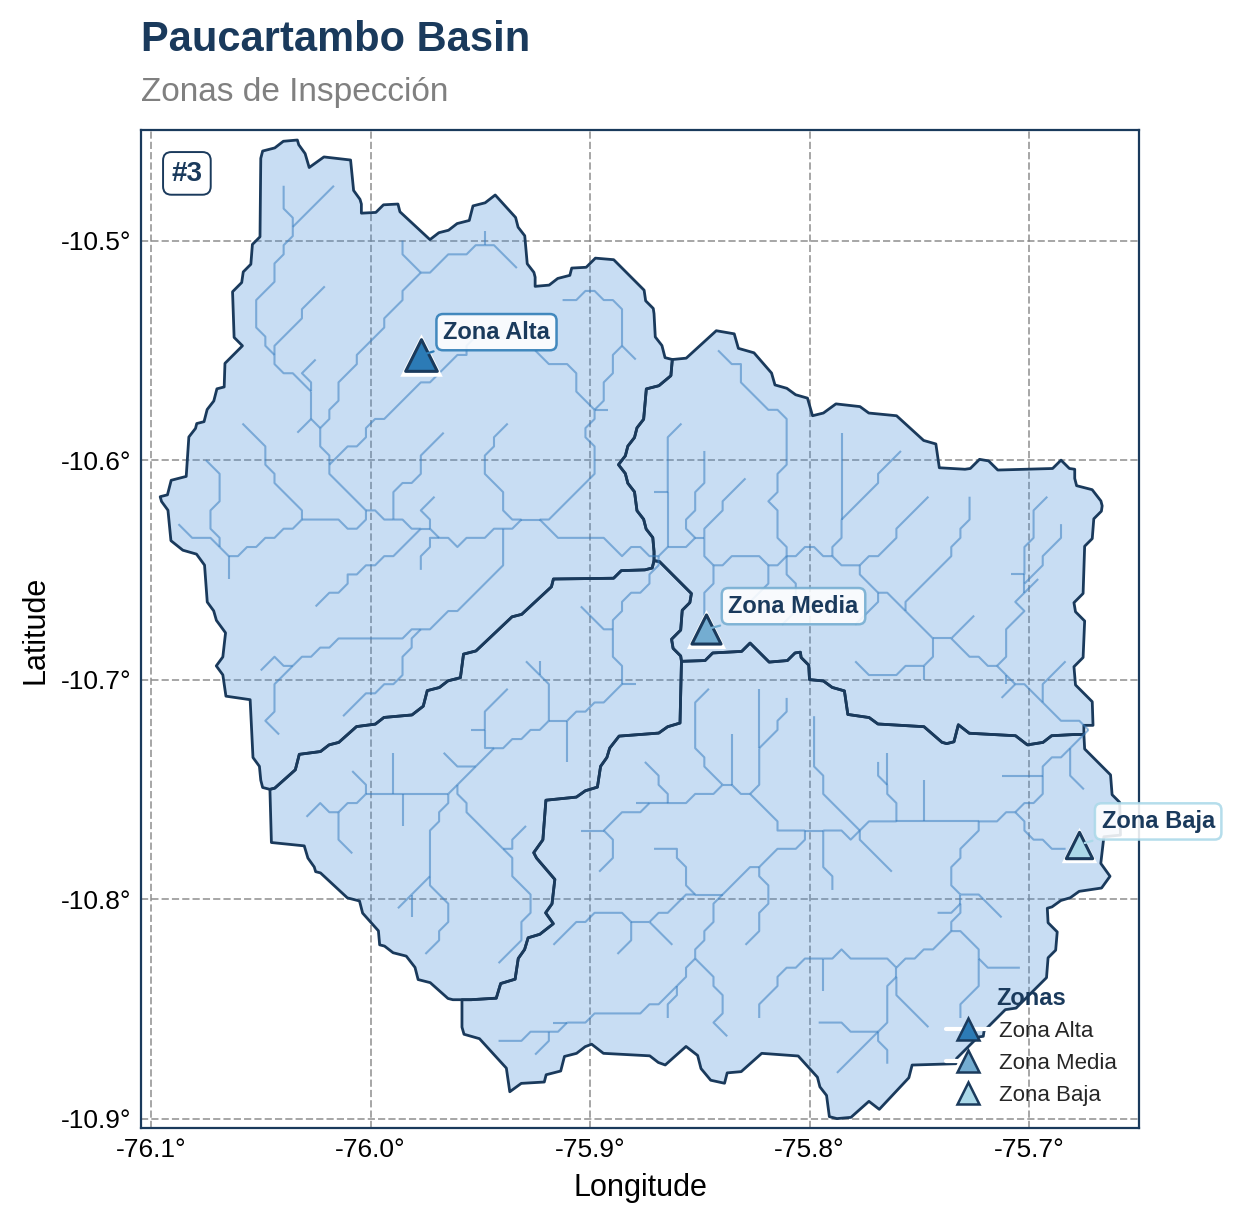
\includegraphics[width=.8\textwidth]{Figures/map4.3.png}
    \caption{Ubicación de estaciones virtuales para las zonas alta (EstAltaWS), media (EstMediaWS) y baja(EstBajaWS) de la cuenca (Fuente: Elaboración Propia)}
    \label{fig:4}
\end{figure}

\subsubsection{Radiación solar y temperatura}

La Figura \ref{fig:4a} presenta la radiación solar promedio mensual en la cuenca
del río Paucartambo, estimada a partir del reanálisis ERA5. Se observa un valor
promedio anual de aproximadamente 20.0 MJ/m\textsuperscript{2}/día, con picos de
24.5 MJ/m\textsuperscript{2}/día durante los meses de verano (enero a marzo). En
invierno (junio a agosto), la radiación aumenta ligeramente hasta alcanzar
valores promedio de 26.0 MJ/m\textsuperscript{2}/día, debido a una mayor
frecuencia de días con cielo despejado y menor nubosidad.

La temperatura mínima promedio mensual se muestra en la Figura \ref{fig:4b}. El
promedio anual es de 5.6\textdegree C en la zona baja y -1.0\textdegree C en la
zona alta. El mes más frío es julio, con valores mínimos promedio de
1.0\textdegree C en la zona baja y -4.0\textdegree C en la zona alta. Las
temperaturas mínimas más elevadas se registran entre enero y marzo, alcanzando
aproximadamente 5.6\textdegree C en la zona baja y -1.0\textdegree C en la zona
alta.

La Figura \ref{fig:4c} presenta la temperatura máxima promedio mensual, con
valores anuales de 16.0\textdegree C en la zona baja y 11.0\textdegree C en la
zona alta. Estas temperaturas muestran una variación reducida a lo largo del
año, reflejando un régimen térmico relativamente constante.

\begin{figure}[H]
    \centering
    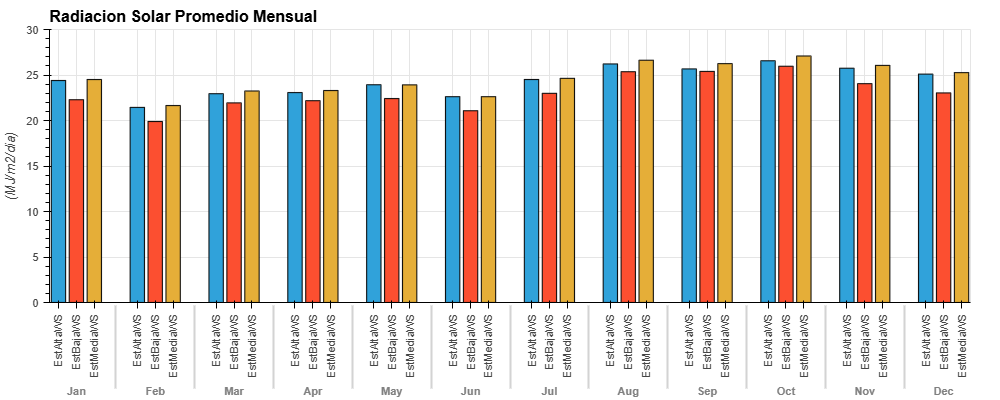
\includegraphics[width=1.0\textwidth]{Figures/bokeh_plot_fig_05.png}
    \caption{Radiación Solar Promedio Mensual usando datos ERA5 Reanálisis para las zonas alta (EstAltaWS), media (EstMediaWS) y baja(EstBajaWS) de la cuenca}
    \label{fig:4a}
\end{figure}

\begin{figure}[H]
    \centering
    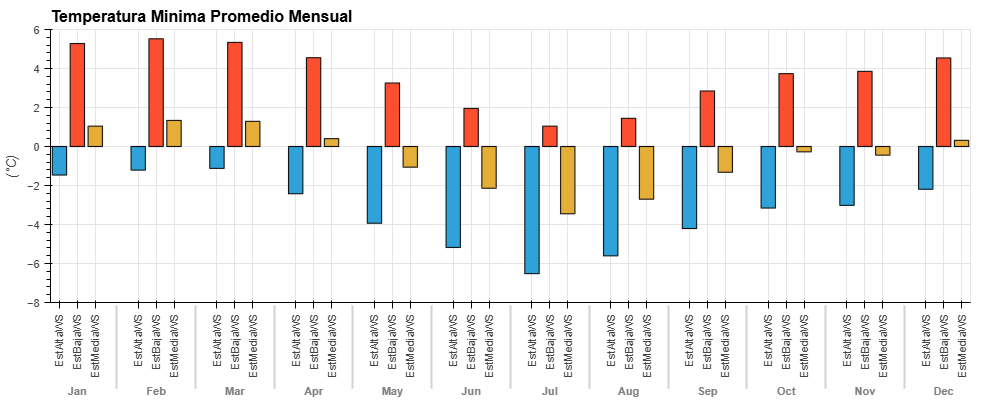
\includegraphics[width=1.0\textwidth]{Figures/bokeh_plot_fig_01.png}
    \caption{Temperatura Mínima Promedio Mensual usando datos ERA5 Reanálisis para las zonas alta (EstAltaWS), media (EstMediaWS) y baja(EstBajaWS) de la cuenca}
    \label{fig:4b}
\end{figure}

\begin{figure}[H]
    \centering
    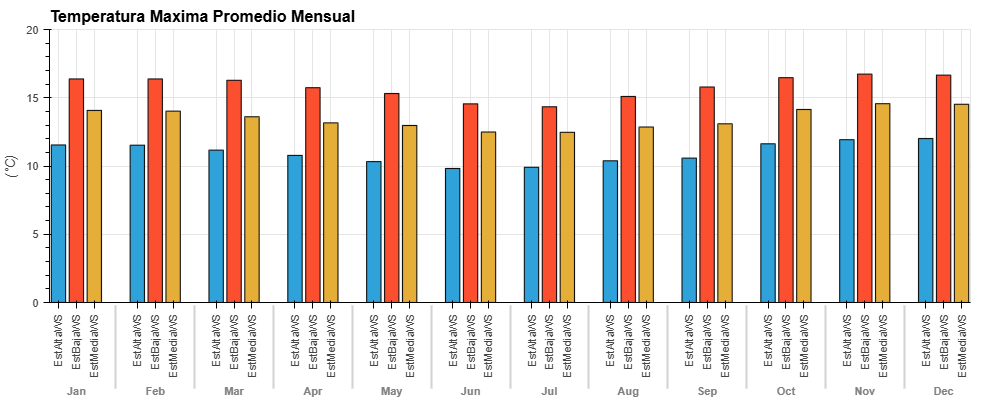
\includegraphics[width=1.0\textwidth]{Figures/bokeh_plot_fig_02.png}
    \caption{Temperatura Máxima Promedio Mensual usando datos ERA5 Reanálisis para las zonas alta (EstAltaWS), media (EstMediaWS) y baja(EstBajaWS) de la cuenca} 
    \captionsetup{labelfont=rm,skip=2pt,textfont=rm,font=small}
    \label{fig:4c}
\end{figure}

\subsubsection{Humedad relativa y velocidad del viento}

La Figura \ref{fig:4d} muestra la humedad relativa promedio mensual en las zonas
alta, media y baja de la cuenca. Se observa que la humedad relativa presenta un
comportamiento elevado y constante a lo largo del año, con valores que oscilan
entre 75.0\% y 95.0\%. Los mayores valores se registran durante los meses de
verano (enero a marzo), mientras que los mínimos se presentan en los meses de
invierno (junio a agosto), en especial en las zonas altas. Esta estabilidad
indica una atmósfera predominantemente húmeda, coherente con la climatología de
la región.

La Figura \ref{fig:4e} presenta la velocidad del viento promedio mensual. Se
observa que los valores más altos se registran en los meses de invierno (junio a
agosto), especialmente en la zona alta, con velocidades promedio cercanas a 3.5
m/s. En contraste, durante los meses de verano (enero a marzo), las velocidades
disminuyen por debajo de 2.0 m/s. Esta variabilidad estacional sugiere un
fortalecimiento del gradiente térmico en invierno, lo cual puede influir en la
dinámica de transporte de humedad y en los procesos de evapotranspiración en la
cuenca.

\begin{figure}[H]
    \centering
    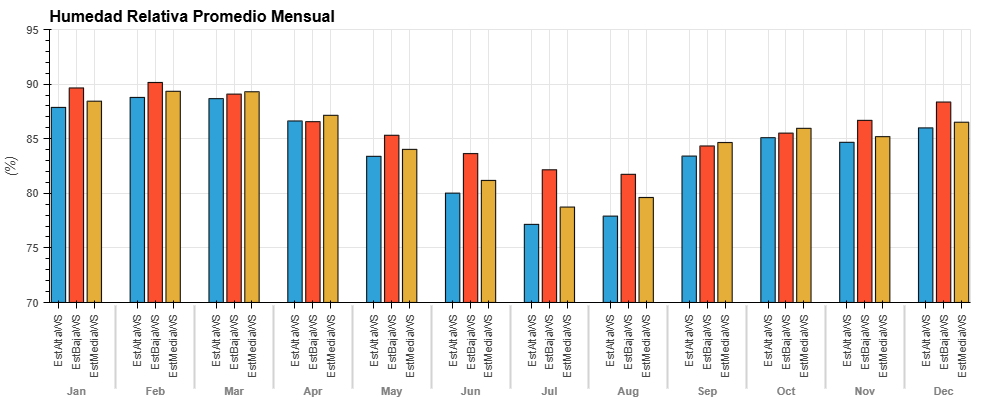
\includegraphics[width=1.0\textwidth]{Figures/bokeh_plot_fig_04.png}
    \caption{Humedad Relativa Promedio Mensual usando datos ERA5 Reanálisis para las zonas alta (EstAltaWS), media (EstMediaWS) y baja(EstBajaWS) de la cuenca}
    \captionsetup{labelfont=rm,skip=2pt,textfont=rm,font=small}
    \label{fig:4d}
\end{figure}

\begin{figure}[H]
    \centering
    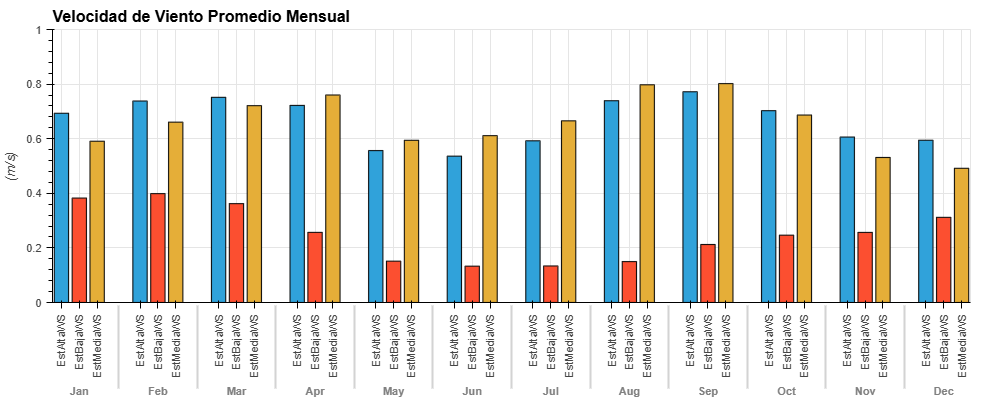
\includegraphics[width=1.0\textwidth]{Figures/bokeh_plot_fig_03.png}
    \caption{Velocidad de Viento Promedio Mensual usando datos ERA5 Reanálisis para las zonas alta (EstAltaWS), media (EstMediaWS) y baja(EstBajaWS) de la cuenca}
    \label{fig:4e}
\end{figure}

\newpage{}
\section{CARACTERIZACIÓN HIDROLÓGICA}

\subsection{HIDROGRAFÍA}

\subsubsection{Caracterización a Nivel Regional}

Según la Resolución Ministerial N.º RM-022-2008-AG de la Autoridad Nacional del
Agua (ANA), la delimitación de unidades hidrográficas en el Perú sigue la
metodología de Pfafstetter \parencite{verdin1999topological}. En este marco, la
cuenca del río Paucartambo forma parte del sistema del río Perené y se ubica en
su zona noroccidental. Limita al norte con la cuenca del río Pachitea y al oeste
con las de los ríos Mantaro y Alto Huallaga. 

\subsubsection{Caracterización a Nivel Local}

El área de estudio comprende las microcuencas que aportan a la Central
Hidroeléctrica Yuncán, con una superficie total de 1583.5 km\textsuperscript{2}.
Estas se localizan en la cuenca alta del río Paucartambo y están delimitadas en
la Figura \ref{fig:4f}.

\begin{figure}[H]
    \centering
    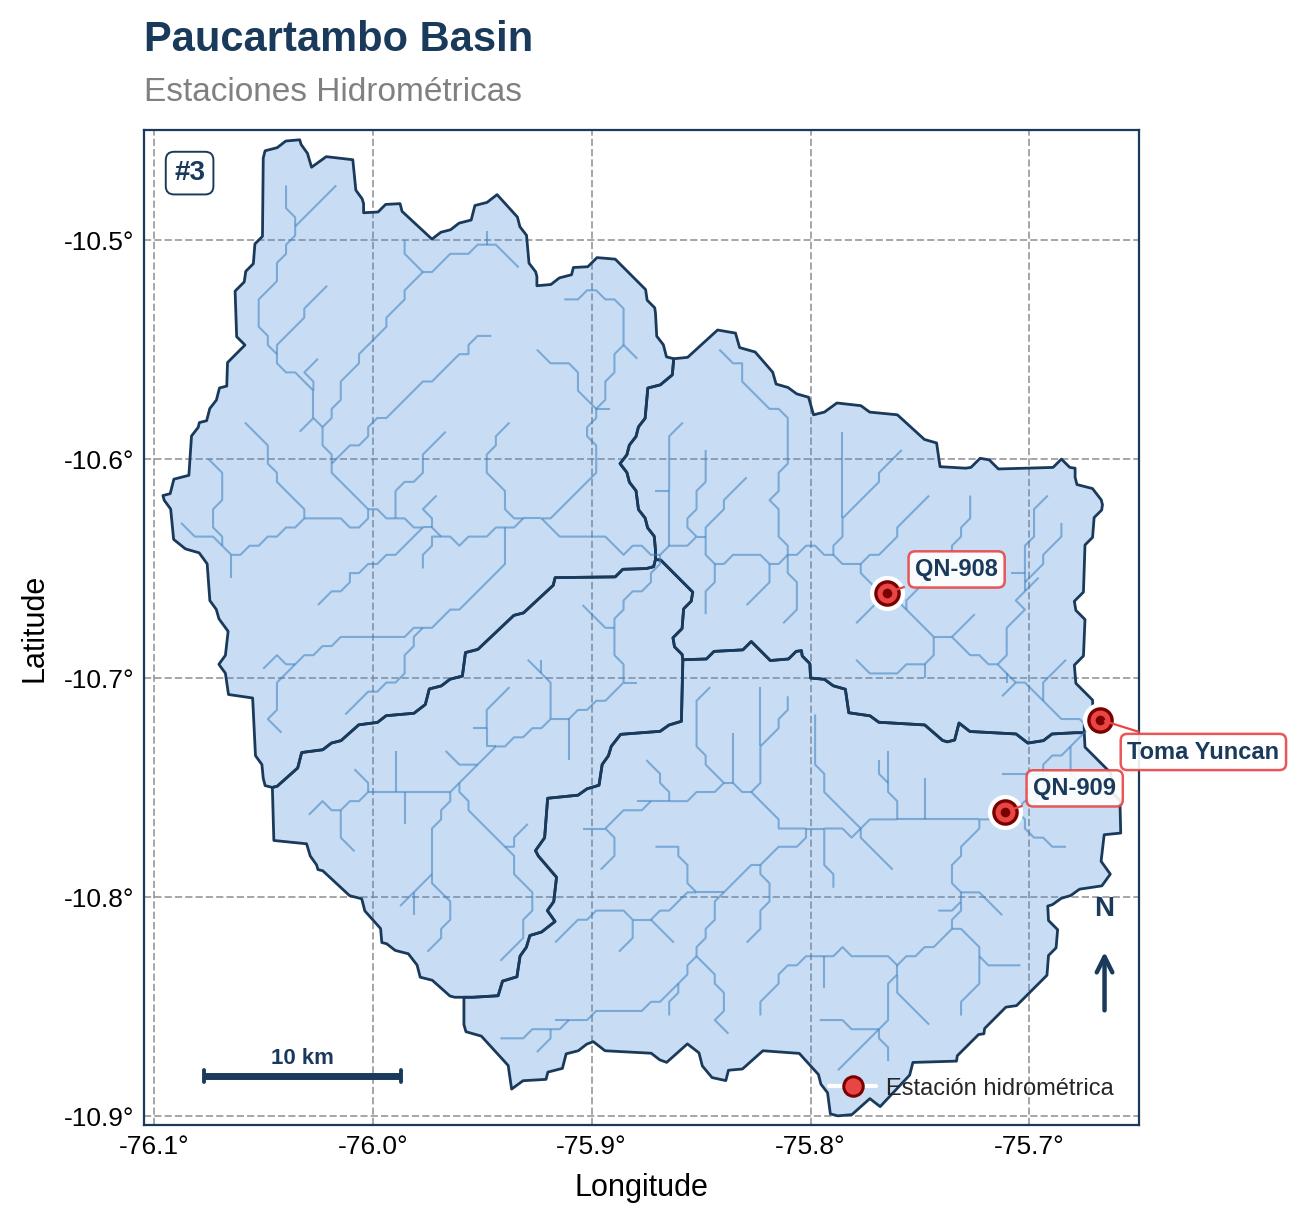
\includegraphics[width=.7\textwidth]{Figures/map4.4.png}
    \caption{Hidrografía regional: ubicación del reservorio Yuncán (QN-906) y de las estaciones hidrológicas asociadas QN-908 (Uchuhuerta), QN-909 (Huallamayo). (Fuente: Elaboración Propia)}
    \captionsetup{labelfont=rm,skip=2pt,textfont=rm,font=small}
    \label{fig:4f}
\end{figure}

\subsection{PARÁMETROS MORFOLÓGICOS DE LA MICRO-CUENCA}
En este capítulo se analizan los principales parámetros morfológicos de las
cuencas ubicadas dentro del área de influencia del proyecto.

\subsubsection*{Área de drenaje}
El área de drenaje corresponde a la superficie que aporta escorrentía hacia un
punto específico de la cuenca. El área total hasta QN-906, correspondiente al
reservorio Yuncán, es de 1583 km\textsuperscript{2}. La subcuenca de Uchuhuerta
abarca 889 km\textsuperscript{2}, mientras que la de Huallamayo comprende 445
km\textsuperscript{2}.

\subsubsection*{Perímetro de la cuenca}
El perímetro es la longitud de la línea divisoria que delimita la cuenca
respecto a cuencas vecinas. Hasta el embalse Yuncán, el perímetro es de 195 km;
hasta Uchuhuerta, 160 km; y hasta Huallamayo, 112 km.

\subsubsection*{Curva hipsométrica}
La curva hipsométrica representa la relación entre altitud y área acumulada.
Permite analizar la distribución del relieve y su influencia en procesos como
escorrentía y almacenamiento superficial. Las Figuras \ref{fig:5a}, \ref{fig:5b}
y \ref{fig:5c} muestran las curvas hipsométricas de las microcuencas del área de
estudio.

\begin{figure}[H]
    \centering
    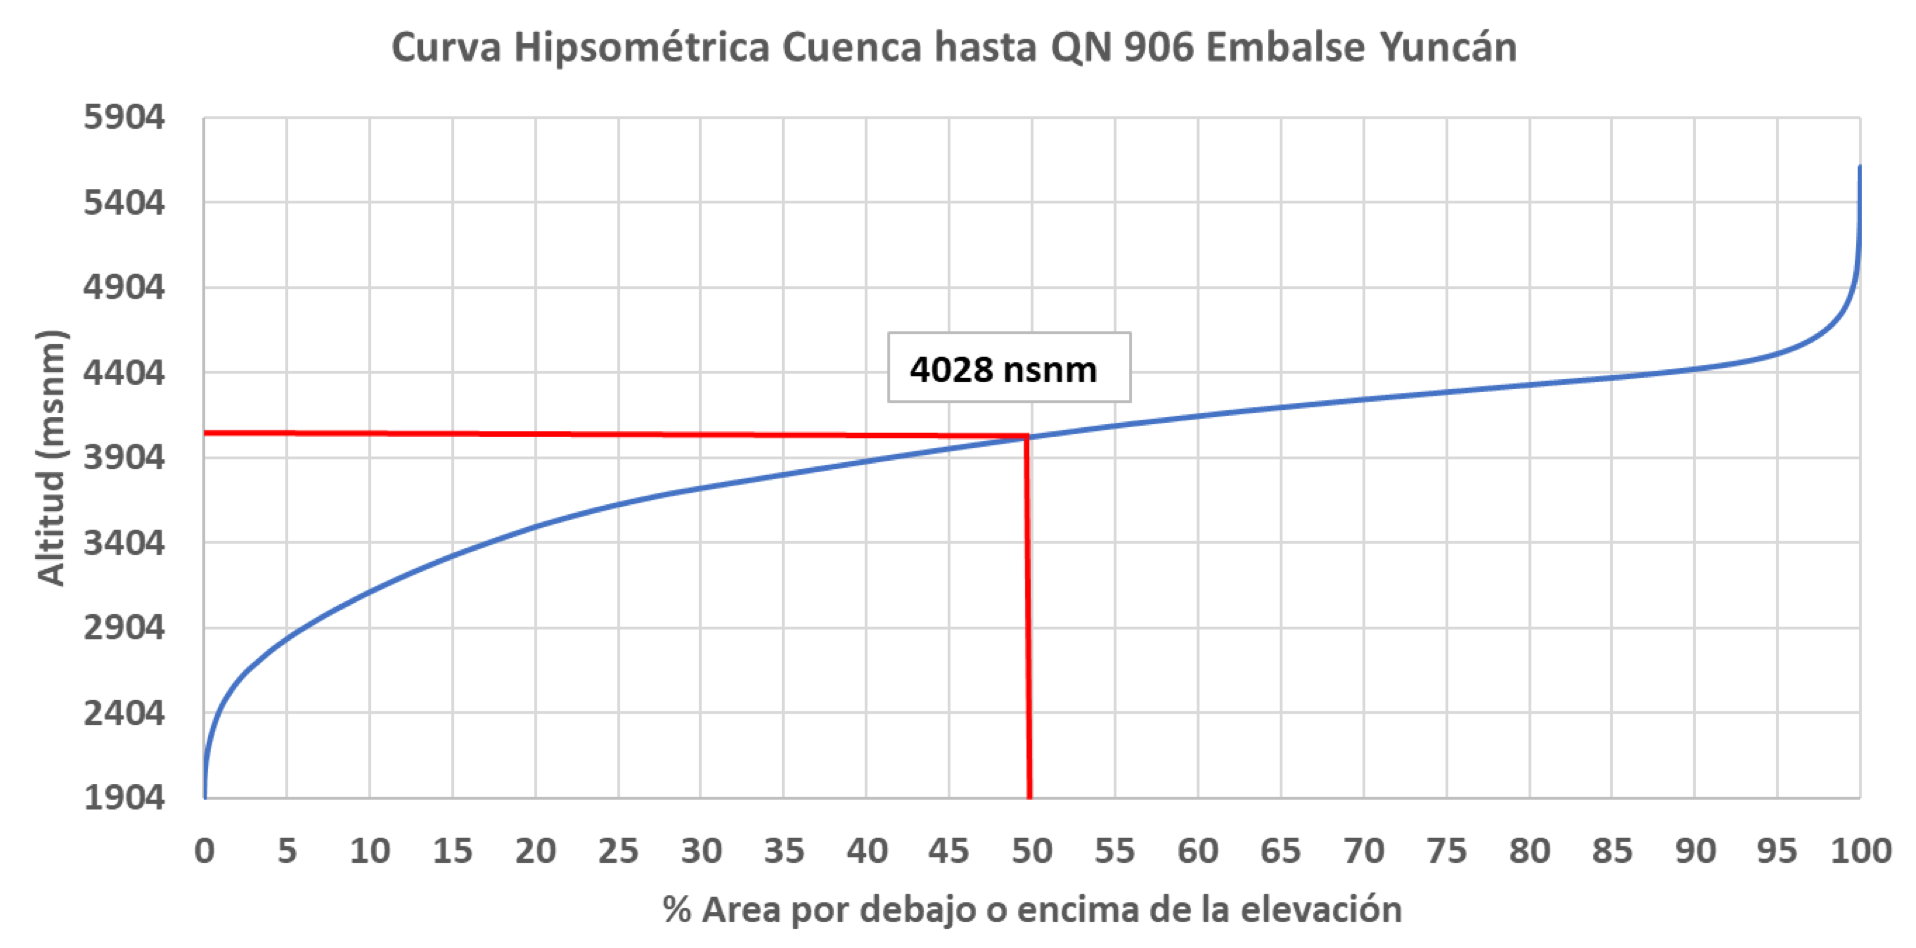
\includegraphics[width=.85\textwidth]{Figures/fig05a.png}
    \caption{Curvas Hipsométrica de la cuenca QN-906}
    \label{fig:5a}
\end{figure}

\begin{figure}[H]
    \centering
    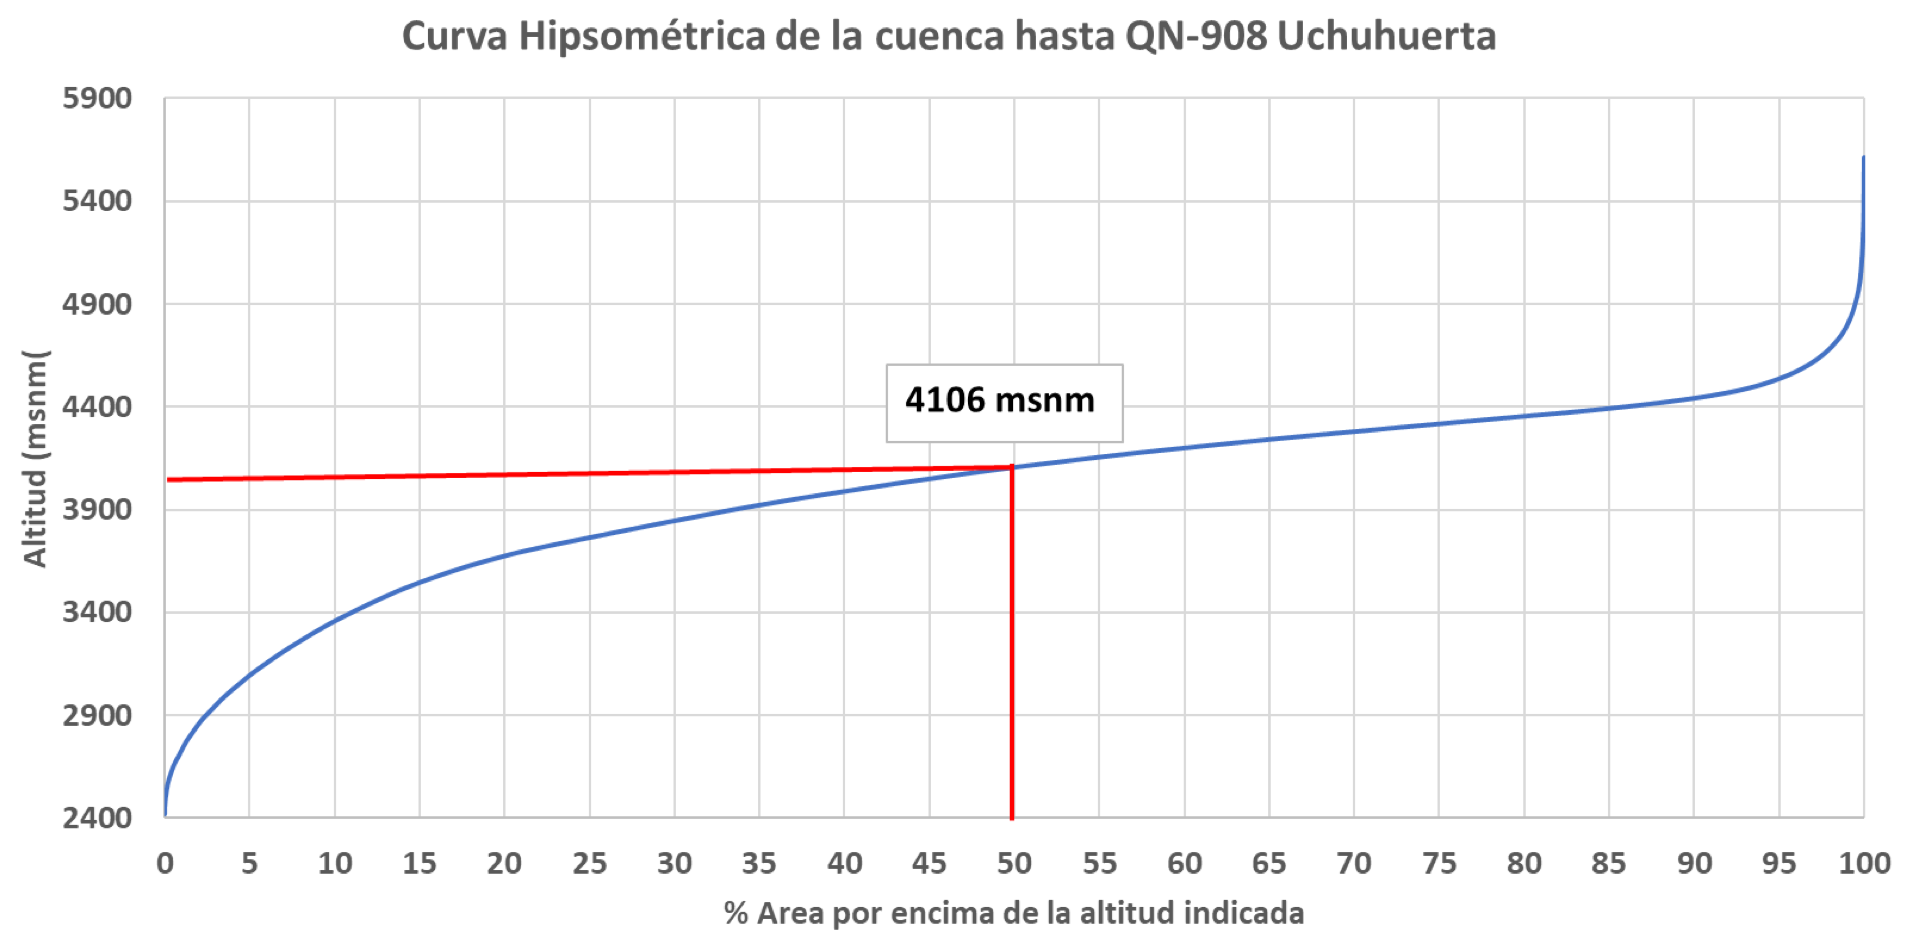
\includegraphics[width=.85\textwidth]{Figures/fig05b.png}
    \caption{Curvas Hipsométrica de la cuenca QN-908}
    \label{fig:5b}
\end{figure}

\begin{figure}[H]
    \centering
    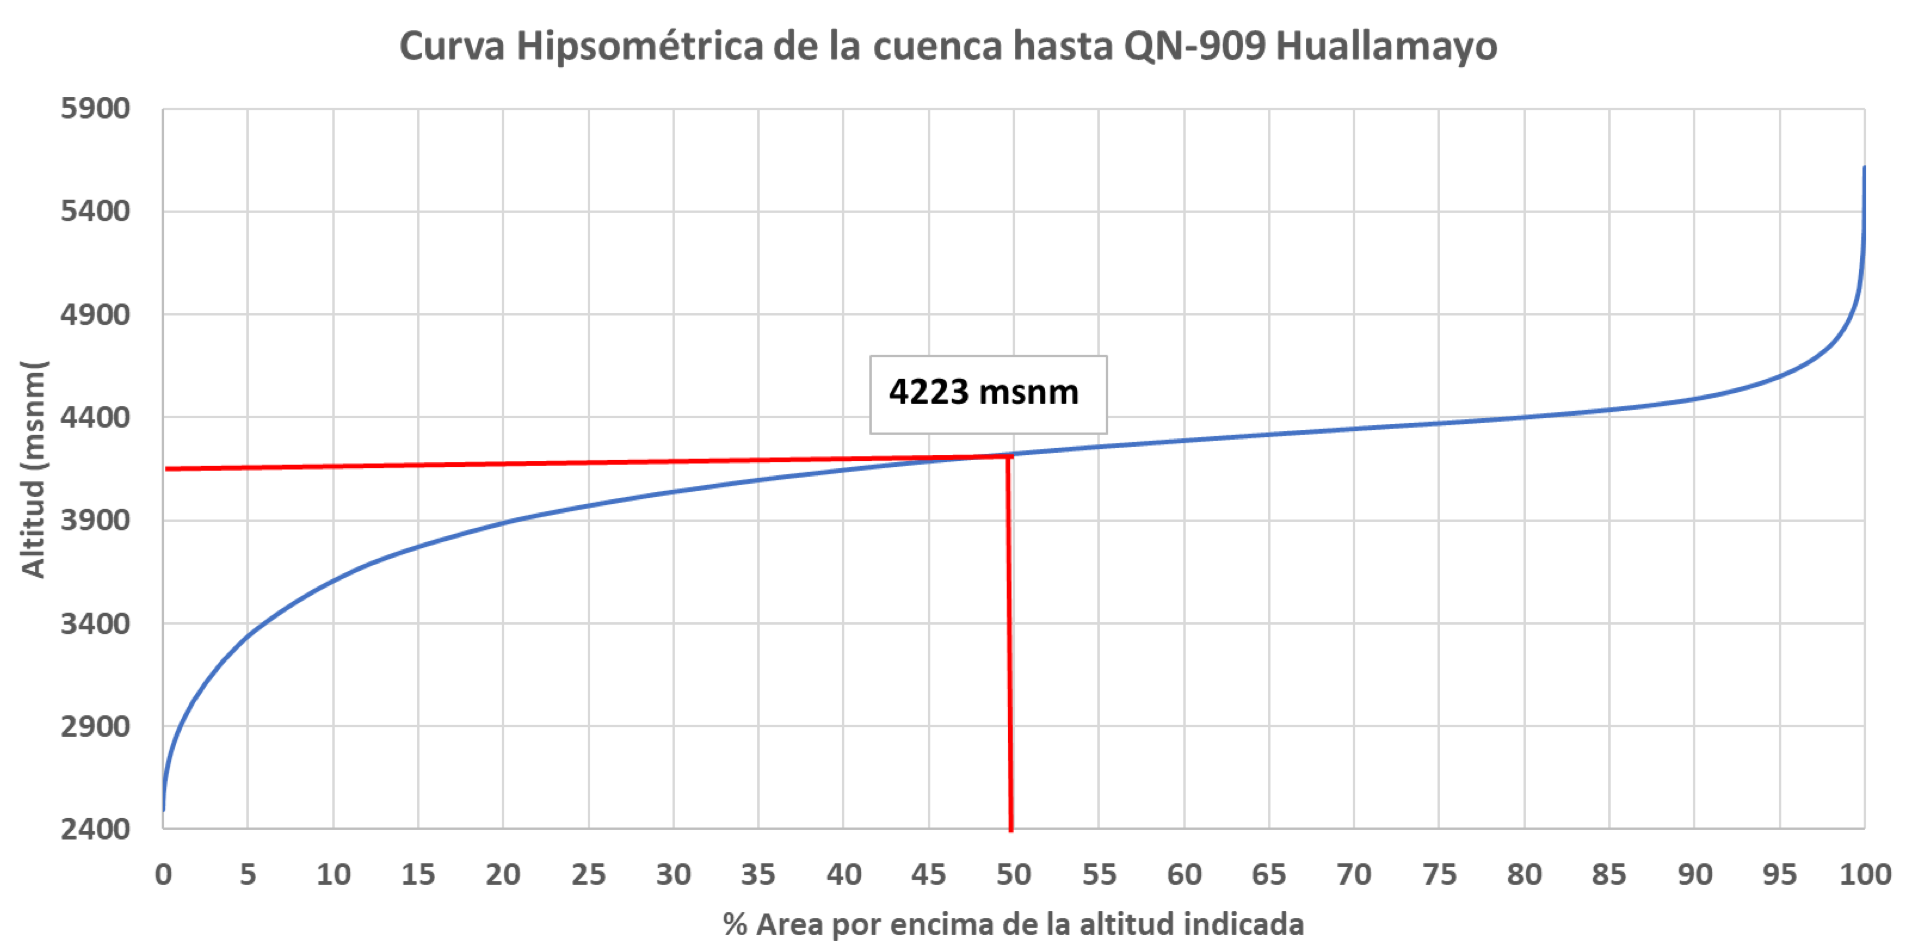
\includegraphics[width=.85\textwidth]{Figures/fig05c.png}
    \caption{Curvas Hipsométrica de la cuenca QN-909}
    \label{fig:5c}
\end{figure}

\subsubsection*{Coeficiente de compacidad (K\textsubscript{c})} El coeficiente
de compacidad o índice de Gravelius permite evaluar la forma de una cuenca. Se
calcula como la relación entre el perímetro $P$ y el área $A$ de la cuenca:

\[
K_c = \frac{0.28 \cdot P}{\sqrt{A}}
\]

Valores superiores a 1.75 indican cuencas con forma alargada u ovalada, como
ocurre en ambos casos analizados.

\subsubsection*{Factor de forma (F\textsubscript{f})} Este parámetro describe la
geometría de la cuenca. Se define como el cociente entre el área $A$ y el
cuadrado de la longitud del cauce principal $L$:

\[
F_f = \frac{A}{L^2}
\]

En el caso de la microcuenca de la quebrada Chonta, con un valor de 0.4, el
factor de forma sugiere baja susceptibilidad a eventos de avenida súbita.

\subsubsection*{Rectángulo equivalente}
El rectángulo equivalente permite aproximar la forma de la cuenca a un
rectángulo de lados $l$ y $L$, determinados a partir del área y el coeficiente
de compacidad. Las expresiones para los lados son:

\[
L = \frac{K_c \sqrt{A}}{1.12 \left[1 - \sqrt{1 - \left(\frac{1.12}{K_c}\right)^2}\right]}
\quad \text{y} \quad
l = \frac{K_c \sqrt{A}}{1.12 \left[1 + \sqrt{1 - \left(\frac{1.12}{K_c}\right)^2}\right]}
\]

\subsubsection*{Pendiente media del río}
La pendiente media del cauce principal se obtiene dividiendo el desnivel entre
su nacimiento ($H_M$) y su desembocadura ($H_m$), por la longitud $L$ del cauce:

\[
i = \frac{H_M - H_m}{L}
\]

En la microcuenca de la quebrada Chonta, la pendiente media es de 8.0\%. Esta
condición topográfica, de carácter medianamente accidentado, limita el
almacenamiento natural en las zonas altas, reduciendo así la eficiencia del
proceso de recarga.

\subsubsection*{Coeficiente de masividad (C\textsubscript{m})} Este índice
relaciona la altitud media $H$ de la cuenca con su superficie $A$, y se expresa
en m/km\textsuperscript{2}:

\[
C_m = \frac{H}{A}
\]
Proporciona una medida del relieve promedio por unidad de área, útil para
evaluar el grado de compactación vertical de la cuenca.

En la siguiente Tabla \ref{tab05} se presenta un resumen de los principales
parámetros morfológicos de la microcuenca de la quebrada Chonta. 

\begin{table}[ht]
\centering
\caption{Parámetros Morfológicos de las Cuencas}
\label{tab05}
\small
\begin{tabular}{l c c c c}
\toprule
\textbf{Parámetro} & \textbf{Qn-905 (Yuncán)} & \textbf{QN-908 (Uchuhuerta)} &
\textbf{QN-909 (Huallamayo)} & \textbf{Unidad} \\
\midrule
Área de la cuenca (A)                           & 1583   & 889    & 1583.0   &
Km\textsuperscript{2} \\
Perímetro de la cuenca (P)                      & 195.0  & 160.0  & 112.0    &
Km \\
Cota Mayor (CM)                                 & 4880   & 5613   & 4841     &
m.s.n.m. \\
Cota Menor (Cm)                                 & 3871   & 2418   & 2418     &
m.s.n.m. \\
Longitud del Cauce Mayor                        & 78     & 60.5   & 40.1     &
Km \\
Coeficiente de Compacidad (K\textsubscript{c})  & 1.4    & 1.5    & 1.5      &
\\
Factor de Forma (F\textsubscript{m})            & 0.3    & 0.2    & 0.3      &
\\
Razón de Circularidad (Rc)                      & 0.5    & 0.4    & 0.4      &
\\
Altitud Media de la Cuenca (L)                  & 3902.9 & 4002.0 & 3742.6   &
m.s.n.m. \\
Lado Mayor (L)                                  & 76.9   & 66.7   & 46.4     &
Km \\
Lado Menor (l)                                  & 20.6   & 13.3   & 9.6      &
Km \\
Pendiente Media del Río (lc)                    & 1\%    & 5\%    & 6\%      &
m/m \\
Coeficiente de Masividad (C\textsubscript{m})   & 2.5    & 4.5    & 2.4      &
m/km\textsuperscript{2} \\
\bottomrule
\end{tabular}
\end{table}

% ─────────────────────────────────────────────────────────────────────────────
\section{ELEMENTOS HIDRÁULICOS DEL SISTEMA DE GENERACIÓN}
\label{section:ElementosHidraulicos}

La C.H.~Yuncán aprovecha las aguas de los ríos Huachón y Paucartambo mediante
dos captaciones: la Bocatoma Uchuhuerta (río Huachón) y el Embalse de Regulación
Huallamayo (río Paucartambo). El agua es conducida a la Casa de Máquinas a
través de una red de túneles y un conducto forzado. La
Tabla~\ref{tab:elementos_hid} resume las características principales de cada
elemento de conducción.

\begin{table}[H]
\centering
\caption{Características técnicas de los elementos hidráulicos de conducción — C.H.~Yuncán.}
\label{tab:elementos_hid}
% \footnotesize
\begin{tabular}{l l S[table-format=5.1] c c}
\toprule
\textbf{Elemento} & \textbf{Tipo} & \textbf{Long. (m)} & \textbf{Diámetro (m)} &
\textbf{Pendiente} \\
\midrule
Túnel 1 (Uchuhuerta) & Pelo libre & 11161.9 & $\varnothing$3.50 (TBM dom.) &
1/600 \\
Túnel 2              & Presión    &  1605.6 & $\varnothing$3.40            &
1/11 -- 1/1\,000 \\
Túnel 3 (Huallamayo) & Presión    &   246.9 & $\varnothing$3.40            &
1/1\,000 + pique 81\,m \\
Túnel 4              & Presión    &  7009.9 & $\varnothing$3.40 (ef.)      &
1/1\,000 \\
Conducto Forzado     & Presión    &   709.3 &
$\varnothing$3.40\,$\to$\,$\varnothing$1.20 & 52° \\
\bottomrule
\end{tabular}
\begin{minipage}{0.85\textwidth}
\vspace{2pt}\scriptsize\textit{Fuente: Características Técnicas de los Elementos
Hidráulicos C.H.~Yuncán. T1 presenta secciones circulares (TBM,
$\varnothing$3.50~m dominante) y herradura; la longitud de T3 (246.92~m) incluye
un pique vertical de 81.33~m. Revestimientos: concreto, shotcrete y tramos sin
revestir en T1; concreto en T2/T3/T4; acero soldado en conducto forzado.}
\end{minipage}
\end{table}

\subsection{TIEMPO DE DESPLAZAMIENTO DESDE HUALLAMAYO HASTA LA CENTRAL}

Los tiempos de desplazamiento fueron calculados para distintos caudales
representativos de estiaje y avenida en el Embalse Huallamayo, aplicando la
relación $v = Q/A$ para los túneles a presión y el conducto forzado.

La Tabla~\ref{tab:tt_hual} presenta los resultados para la ruta de análisis
(Embalse Huallamayo~→ Casa de Máquinas, $\approx$7\,966~m), íntegramente a
presión.

\begin{table}[H]
\centering
\caption{Tiempo de desplazamiento Embalse Huallamayo → Casa de Máquinas (T3+T4+Conducto Forzado).}
\label{tab:tt_hual}
% \small
\begin{tabular}{c l S[table-format=1.2] S[table-format=1.2] S[table-format=1.2] S[table-format=1.2]}
\toprule
\textbf{Q} & \textbf{Época} & \textbf{T3 (h)} & \textbf{T4 (h)} & \textbf{CF
(h)} & \textbf{Total (h)} \\
\textbf{(m\textsuperscript{3}/s)} & & & & & \\
\midrule
 3  & Estiaje          & 0.21 & 5.89 & 0.29 & 6.39 \\
10  & Transición        & 0.06 & 1.77 & 0.09 & 1.92 \\
20  & Avenida           & 0.03 & 0.88 & 0.04 & 0.95 \\
30  & Avenida máx.\     & 0.02 & 0.59 & 0.03 & 0.64 \\
\bottomrule
\end{tabular}
\begin{minipage}{0.92\textwidth}
\small\textit{T3: Túnel 3 (incluye pique vertical 81~m); T4: Túnel 4; CF:
Conducto Forzado. Caudales representativos derivados de la serie simulada
QN-909.}
\end{minipage}
\end{table}

Los tiempos resultantes para el Embalse Huallamayo oscilan entre \textbf{0.64 y
6.4~h} para caudales de 30 a 3~m\textsuperscript{3}/s, respectivamente, según
la serie QN-909.

\section{SIMULACIÓN HIDROLÓGICA CON EL MODELO VIC}

\subsection{DOMINIO DEL MODELO E INFORMACIÓN PLUVIOMÉTRICA}

\subsubsection{Descripción General}

Para la estimación de los caudales naturales de la cuenca del río Paucartambo,
se empleó el modelo hidrológico distribuido VIC (Variable Infiltration
Capacity) \parencite{liang1994simple}, ampliamente utilizado en estudios
hidrológicos a escala de cuenca y regional. El modelo VIC resuelve el balance
hídrico en una malla regular de celdas geográficas, representando de manera
explícita procesos de infiltración, evapotranspiración, escorrentía superficial
y flujo base. El modelo opera a escala diaria y requiere como forzantes
meteorológicos variables tales como precipitación, temperatura máxima y mínima,
y velocidad del viento, compatibles con los productos CHIRPS y ERA5-Land
descritos en las secciones anteriores. Adicionalmente, VIC requiere información
estática de la superficie, incluyendo parámetros de suelo, cobertura y uso del
suelo, topografía y características de la vegetación, necesarios para
representar adecuadamente los procesos hidrológicos en cada celda del dominio.

La ecuación fundamental del balance hídrico en el modelo VIC es:

\[
\frac{\partial W}{\partial t} = P - ET - Q_{sup} - Q_{base}
\]

Donde:

\begin{itemize}
    \item $W$ es el almacenamiento total de agua en el suelo [mm],
    \item $P$ es la precipitación [mm/día],
    \item $ET$ es la evapotranspiración real [mm/día],
    \item $Q_{sup}$ es la escorrentía superficial generada por saturación
    [mm/día],
    \item $Q_{base}$ es el flujo base desde la capa de suelo inferior [mm/día].
\end{itemize}

La generación de escorrentía superficial se rige por la curva de capacidad de
infiltración variable, que determina la fracción del área de cada celda que
contribuye a la escorrentía en función del estado de humedad del suelo. El flujo
base es calculado mediante un esquema de drenaje no lineal desde la capa de
suelo profundo. La evapotranspiración potencial se estima mediante el método de
Penman-Monteith, recomendado por la FAO \parencite{allen1998crop}.

El modelo fue configurado sobre una malla espacial con resolución de
aproximadamente 0.009° × 0.009° (~0.9 km). Para cada celda se definieron
parámetros de suelo (textura, porosidad, conductividad hidráulica) y vegetación
(cobertura, índice de área foliar, profundidad radicular), derivados de fuentes
cartográficas oficiales.

Las variables geomorfológicas incorporadas incluyeron topografía, delimitación
de cuencas, tipos de suelo y usos del terreno, procesados y adaptados conforme a
los requerimientos del modelo VIC.

\subsubsection{Definición de la Zona de Estudio Hidrológico}

El ámbito de estudio hidrológico se sitúa principalmente dentro de la cuenca del
río Paucartambo. La malla del modelo VIC fue recortada al dominio de la cuenca
con una resolución de aprox. 1 km, lo que permitió representar de manera
distribuida los procesos hidrológicos en cada celda. Los resultados del modelo
servirán para evaluar las interacciones entre los diferentes componentes del
balance hídrico (ver Figura \ref{fig:2a}, delimitación del área de estudio).

\subsubsection{Características de los Suelos}

La caracterización de suelos se realizó a partir del producto global
\href{https://openlandmap.org}{OpenLandMap Soil Texture Classes (USDA)}, con
resolución espacial de 250 m \parencite{hengl2018soiltexture}. Para el dominio
de la cuenca del río Paucartambo se empleó la capa superficial correspondiente a
0 cm de profundidad, la cual fue recortada al límite de la cuenca y
reclasificada de acuerdo con el sistema textural USDA.

La Figura~\ref{fig:7a} muestra que la clase textural dominante en la cuenca es
\textit{Loam}, con presencia localizada de \textit{Sandy Loam}, principalmente
en sectores altos y de transición, y áreas menores de \textit{Sandy Clay Loam}
y \textit{Clay Loam}. Esta distribución indica un predominio de suelos de
textura media, con capacidad de infiltración y almacenamiento de humedad
moderadas, mientras que las clases con mayor proporción de arena tienden a
favorecer una respuesta hidrológica más rápida y menor retención de agua. Las
clases con mayor contenido de arcilla, aunque poco extensas, pueden presentar
menor conductividad hidráulica y mayor capacidad de almacenamiento.

Para la configuración del modelo VIC, las clases texturales USDA fueron
utilizadas como base para asignar o derivar los parámetros hidráulicos de cada
celda, incluyendo fracciones de arena, limo y arcilla, capacidad de agua
disponible y conductividad hidráulica saturada. La Tabla~\ref{tab06} resume las
clases identificadas y su interpretación hidrológica general dentro del área de
estudio.

\begin{table}[ht]
\centering
\caption{Clases texturales USDA identificadas a partir de OpenLandMap y su interpretación hidrológica para el modelo VIC.}
\label{tab06}
\small
\begin{tabular}{p{0.25\textwidth} p{0.28\textwidth} p{0.35\textwidth}}
\toprule
\textbf{Clase textural USDA} & \textbf{Distribución en la cuenca} &
\textbf{Implicancia hidrológica general} \\
\midrule
\textit{Loam} & Clase predominante en la mayor parte del dominio &
Textura media; infiltración, drenaje y almacenamiento de humedad moderados. \\
\textit{Sandy Loam} & Presencia localizada en sectores altos y zonas de
transición & Mayor proporción de arena; infiltración relativamente alta y menor
retención de humedad. \\
\textit{Sandy Clay Loam} & Áreas puntuales dentro de la cuenca & Comportamiento
intermedio, con mayor retención que los suelos arenosos y drenaje moderado. \\
\textit{Clay Loam} & Áreas menores y localizadas & Mayor proporción de arcilla;
menor conductividad hidráulica relativa y mayor capacidad de almacenamiento. \\
\bottomrule
\end{tabular}
\end{table}

Donde:
\begin{itemize}
    \item \textit{Loam}: suelo franco, con proporciones equilibradas de arena,
    limo y arcilla.
    \item \textit{Sandy Loam}: suelo franco arenoso, con mayor participación de
    arena.
    \item \textit{Sandy Clay Loam}: suelo franco arcillo arenoso, con mezcla de
    arena y arcilla.
    \item \textit{Clay Loam}: suelo franco arcilloso, con mayor influencia de
    arcilla.
\end{itemize}

Los parámetros de suelo fueron adaptados a la resolución de trabajo del modelo
VIC mediante el remuestreo y agregación de la información de OpenLandMap. La
distribución espacial de estas clases texturales se presenta en la
Figura~\ref{fig:7a}.

\begin{figure}[H]
    \centering
    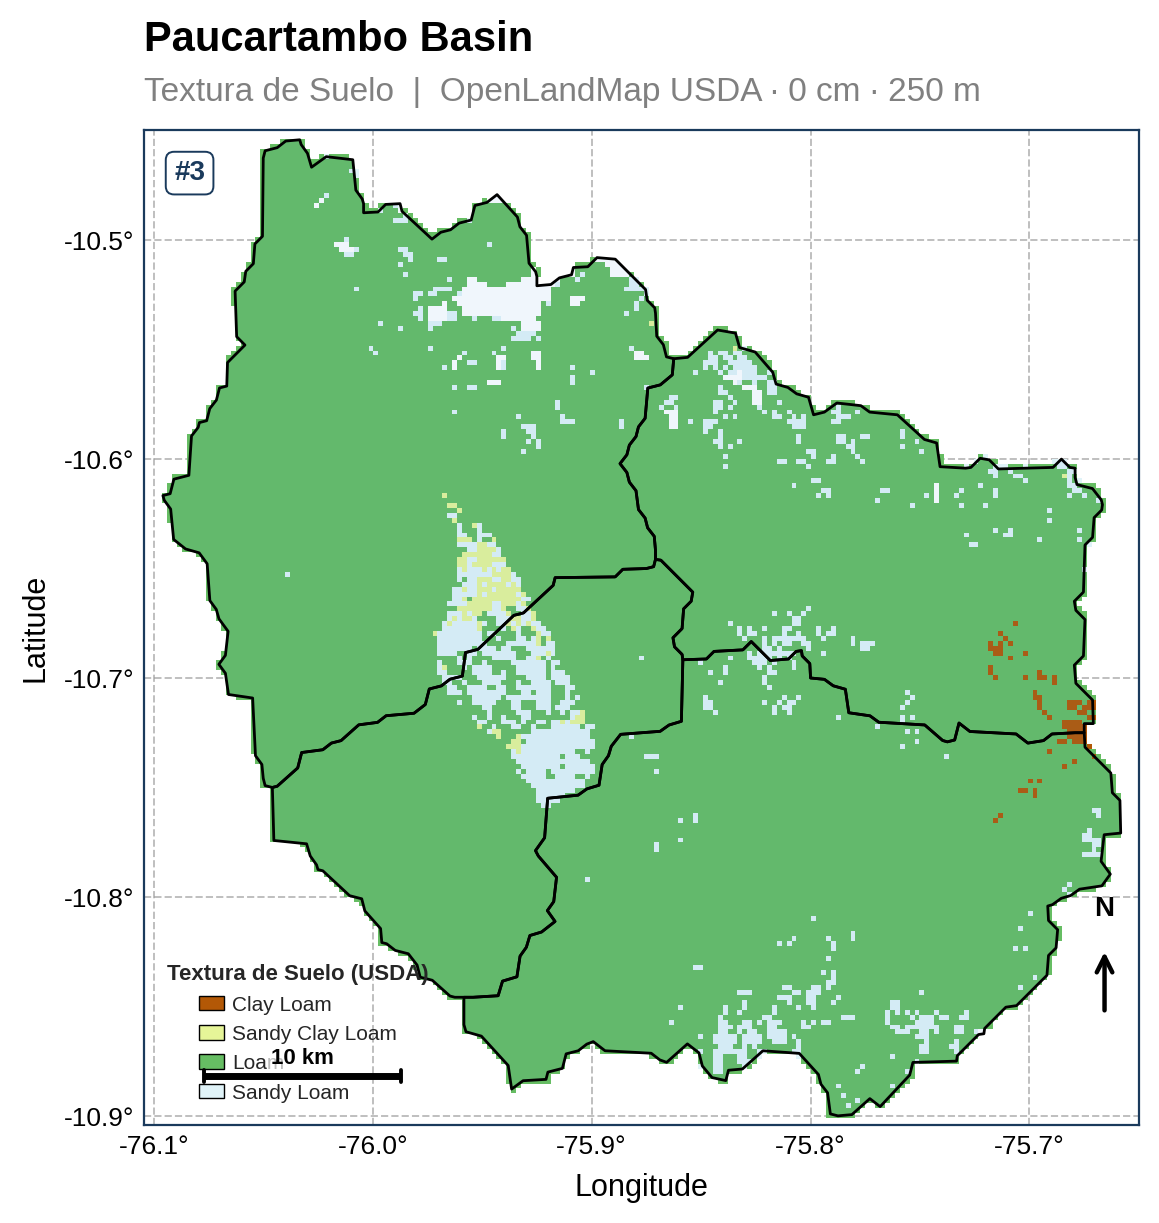
\includegraphics[width=.70\textwidth]{Figures/fig07.png}
    \caption{Mapa de textura de suelo USDA derivado de OpenLandMap a 250 m para la cuenca del río Paucartambo.}
    \label{fig:7a}
\end{figure}

\subsubsection{Mapa de Cobertura y Uso de Suelo}

La cobertura y uso del suelo de la cuenca fue caracterizada a partir del
producto ESA WorldCover v200 correspondiente al año 2021, con resolución
espacial de 10 m \parencite{zanaga2022worldcover}. Esta información fue
recortada al dominio de la cuenca y reclasificada para representar las
principales unidades de cobertura requeridas en la configuración del modelo
hidrológico VIC.

De acuerdo con la Figura~\ref{fig:8a}, la cobertura dominante en la cuenca del
río Paucartambo corresponde a \textit{Grassland}, distribuida de manera extensa
en las zonas altas y medias. En la parte oriental y en sectores asociados a
quebradas y laderas húmedas se observa una mayor presencia de \textit{Tree
Cover}, lo que sugiere áreas con mayor interceptación, rugosidad superficial y
capacidad de regulación hídrica. También se identifican coberturas puntuales de
\textit{Shrubland}, \textit{Bare/Sparse Vegetation}, \textit{Cropland},
\textit{Built-up}, cuerpos de \textit{Permanent Water}, \textit{Herbaceous
Wetland}, \textit{Moss and Lichen} y pequeñas áreas de \textit{Snow and Ice}.

Para fines de modelación, las clases de ESA WorldCover fueron utilizadas como
base para asignar parámetros de vegetación y superficie en cada celda del
modelo, incluyendo albedo, índice de área foliar, profundidad radicular y
características del dosel. La Tabla~\ref{tab:parametros_vegetacion} resume la
interpretación hidrológica general de las clases de cobertura identificadas en
el área de estudio.

\begin{table}[ht]
\centering
\caption{Clases de cobertura ESA WorldCover identificadas en la cuenca y su interpretación hidrológica para el modelo VIC.}
\label{tab:parametros_vegetacion}
\small
\begin{tabular}{p{0.24\textwidth} p{0.30\textwidth} p{0.34\textwidth}}
\toprule
\textbf{Clase ESA WorldCover} & \textbf{Distribución en la cuenca} &
\textbf{Implicancia hidrológica general} \\
\midrule
\textit{Grassland} & Clase dominante en zonas altas y medias &
Cobertura herbácea con interceptación moderada y respuesta hidrológica rápida
en laderas. \\
\textit{Tree Cover} & Concentrada principalmente en el sector oriental y
quebradas húmedas & Mayor interceptación, evapotranspiración y regulación de la
escorrentía superficial. \\
\textit{Shrubland} & Presencia dispersa y localizada & Cobertura arbustiva con
interceptación y rugosidad intermedias. \\
\textit{Bare/Sparse Vegetation} & Sectores puntuales de baja cobertura vegetal &
Menor protección superficial, con mayor susceptibilidad a escorrentía directa y
erosión. \\
\textit{Cropland} y \textit{Built-up} & Áreas reducidas y localizadas & Zonas
con mayor intervención antrópica y modificación local de infiltración y
escorrentía. \\
\textit{Permanent Water}, \textit{Herbaceous Wetland}, \textit{Moss and
Lichen}, \textit{Snow and Ice} & Coberturas menores dentro del dominio &
Unidades hidrológicamente relevantes por almacenamiento superficial, humedad
persistente o condiciones de alta montaña. \\
\bottomrule
\end{tabular}
\end{table}

\begin{figure}[H]
    \centering
    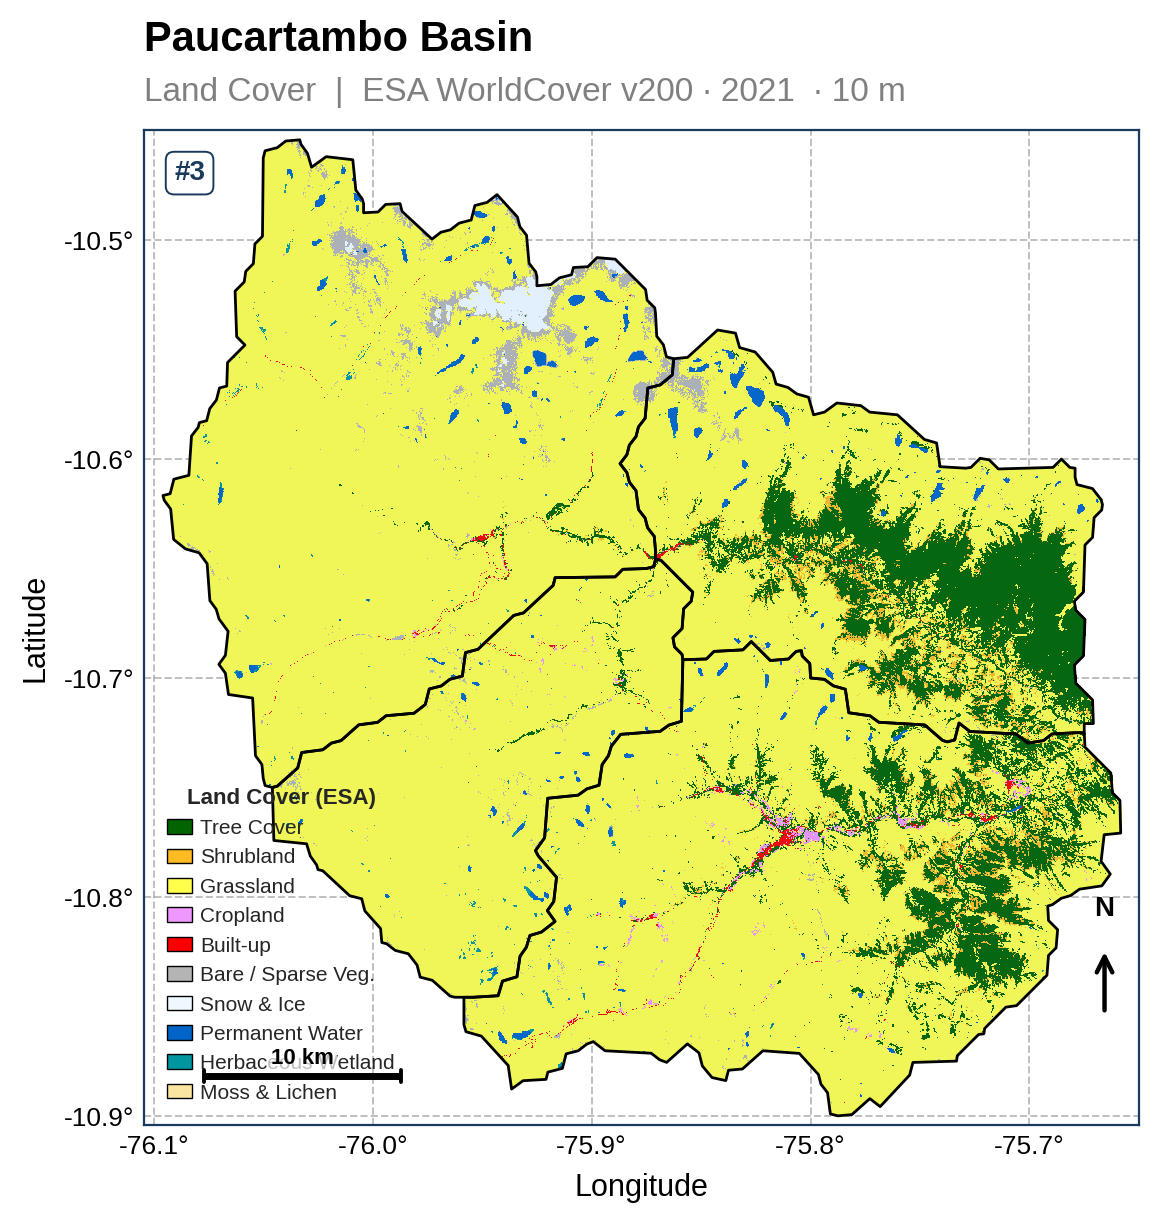
\includegraphics[width=.7\textwidth]{Figures/fig08.png}
    \caption{Mapa de cobertura y uso del suelo derivado de ESA WorldCover v200 (2021) a 10 m para la cuenca del río Paucartambo.}
    \label{fig:8a}
\end{figure}

\subsubsection*{Mapa de Pendientes}

La pendiente del terreno fue derivada a partir del modelo digital de elevación
SRTM, utilizado como base topográfica para caracterizar el relieve de la cuenca.
El DEM fue recortado al dominio de estudio y procesado para calcular la
pendiente en porcentaje \parencite{farr2007srtm}, posteriormente clasificada en
intervalos de 0--10\%, 10--20\%, 20--40\%, 40--60\%, 60--80\% y 80--100\%,
conforme se muestra en la Figura~\ref{fig:9a}.

La distribución espacial evidencia una cuenca con relieve marcadamente
accidentado, donde predominan laderas de pendiente media a alta. Las pendientes
más suaves (0--20\%) se concentran principalmente en fondos de valle, divisorias
locales y pequeñas superficies de menor inclinación, mientras que las clases
superiores a 40\% se distribuyen ampliamente en laderas y quebradas encajonadas.
Estas condiciones topográficas favorecen una respuesta hidrológica rápida,
incrementan el potencial de escorrentía superficial y reducen la capacidad de
retención e infiltración en las zonas más escarpadas.

La Figura~\ref{fig:9a} también muestra la ubicación de estaciones hidrométricas
relevantes dentro del dominio, incluyendo QN-908, QN-909 y la toma Yuncán, lo
que permite relacionar la configuración topográfica de la cuenca con los puntos
de control utilizados en la evaluación hidrológica.

\begin{figure}[H]
    \centering
    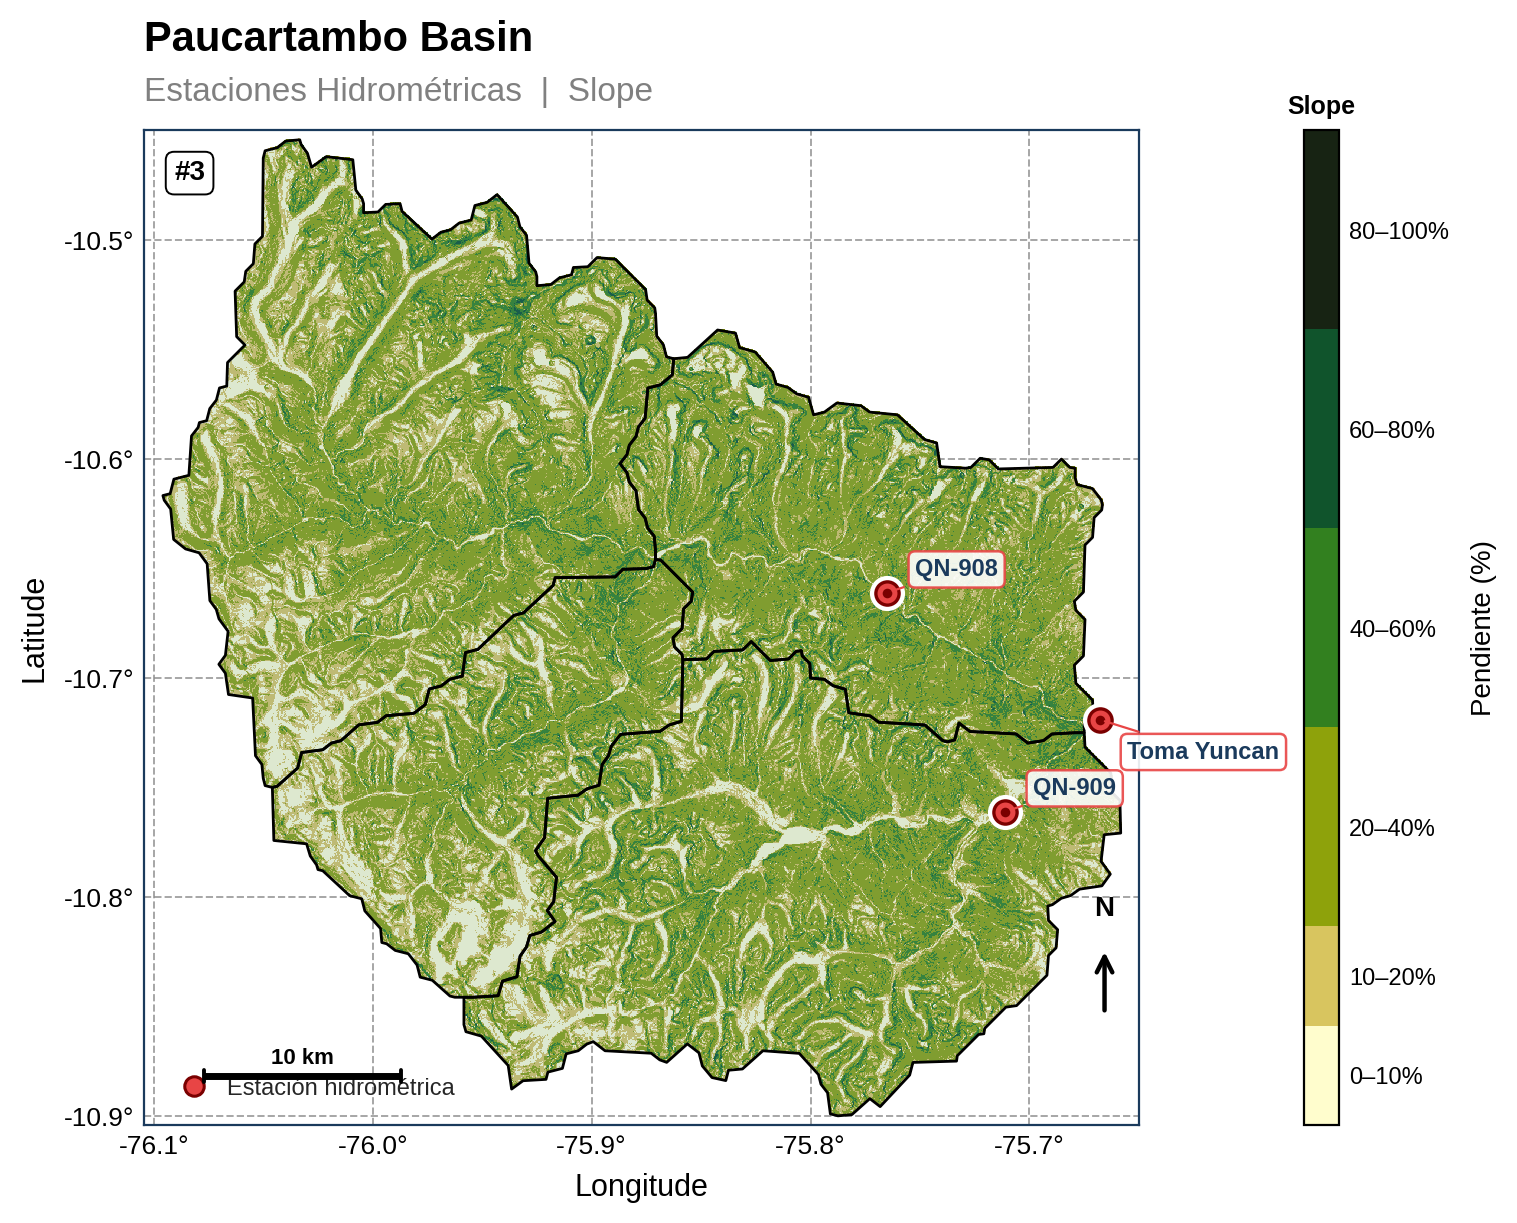
\includegraphics[width=.9\textwidth]{Figures/fig09.png}
    \caption{Mapa de pendientes derivado del DEM SRTM para la cuenca del río Paucartambo y ubicación de estaciones hidrométricas.}
    \label{fig:9a}
\end{figure}

\subsection{CORRECCIÓN POR SESGO}

Como etapa complementaria a la simulación hidrológica, se aplicó una corrección
post-procesamiento a las series de caudales generadas por el modelo VIC mediante
un ajuste por desviación de sesgo (\textit{bias correction}). Este enfoque
permite reducir sesgos sistemáticos e inconsistencias residuales entre los
caudales simulados y los observados, sin modificar la estructura física del
modelo.

El ajuste fue realizado utilizando las series temporales de caudales simulados y
observados en las estaciones con registro disponible. A partir de la comparación
entre ambas series, se estimó la desviación de sesgo para cada punto de control
y se aplicaron factores de corrección orientados a mejorar la representatividad
de los caudales simulados frente a las observaciones.

Los resultados presentados en las secciones siguientes corresponden a las series
de caudales posteriores a la corrección por sesgo; por lo tanto, los valores
expuestos ya consideran el ajuste por desviación de sesgo aplicado a las salidas
del modelo VIC.

\subsection{RESULTADOS DE LAS SIMULACIONES}

\subsubsection{Simulación Hidrológica}
Las simulaciones hidrológicas se realizaron para el período comprendido entre
enero de 1998 y diciembre de 2025, utilizando datos satelitales y de reanálisis
corregidos y adaptados para representar adecuadamente las condiciones climáticas
locales.

\begin{itemize}[leftmargin=1.5em]
    \item La precipitación diaria se obtuvo del conjunto CHIRPS y fue corregida
    mediante la metodología de \textit{quantile mapping}, con el fin de reducir
    sesgos sistemáticos y mejorar su representatividad frente a observaciones
    locales.
    \item Las variables meteorológicas diarias —temperatura máxima y mínima
    (°C), humedad relativa (\%), radiación solar (MJ/m\textsuperscript{2}/día) y
    velocidad del viento (m/s)— provienen del reanálisis ERA5-Land, con
    cobertura desde 1981 hasta 2025.
    \item Para estabilizar las condiciones hidrológicas del modelo, se utilizó
    un período de \textit{spin-up} de 4 años, completando la precipitación
    mediante la repetición cíclica de los primeros años disponibles de la serie
    corregida.
\end{itemize}

El modelo \textbf{VIC} fue ejecutado de forma continua desde el 1 de enero de
1998 hasta el 31 de diciembre de 2025. El período 1998--2002 fue destinado al
\textit{spin-up}, es decir, a la estabilización de las condiciones internas del
modelo (principalmente el contenido de humedad del suelo). A partir de 2002, los
resultados se consideraron válidos para el análisis hidrológico.

Las salidas del modelo VIC representan láminas de escorrentía en milímetros por
celda. Para obtener los caudales en m\textsuperscript{3}/s en los puntos de
control, se aplicó un proceso de routing hidrológico que acumula y enruta estos
valores a lo largo de la red de drenaje hasta cada punto de aforo.

\subsubsection{Caudales Incrementales Promedio Mensuales}

\paragraph{6.2.2.1\quad QN-908 Uchuhuerta}\mbox{}\\
\addcontentsline{toc}{subsubsection}{6.2.2.1 \quad QN-908 Uchuhuerta}
La Figura \ref{fig:9a1}  presenta el hidrograma mensual promedio simulado por el
modelo VIC para la estación QN-908 Uchuhuerta, correspondiente al período
comprendido entre enero de 2002 y diciembre de 2025. Los resultados se comparan
con los caudales observados. Según el análisis estadístico mostrado en la Tabla
\ref{tab:swat_qn908}, ambas series presentan un buen nivel de concordancia,
indicando que las simulaciones reproducen adecuadamente el comportamiento
hidrológico observado.
\begin{figure}[H]
    \centering
    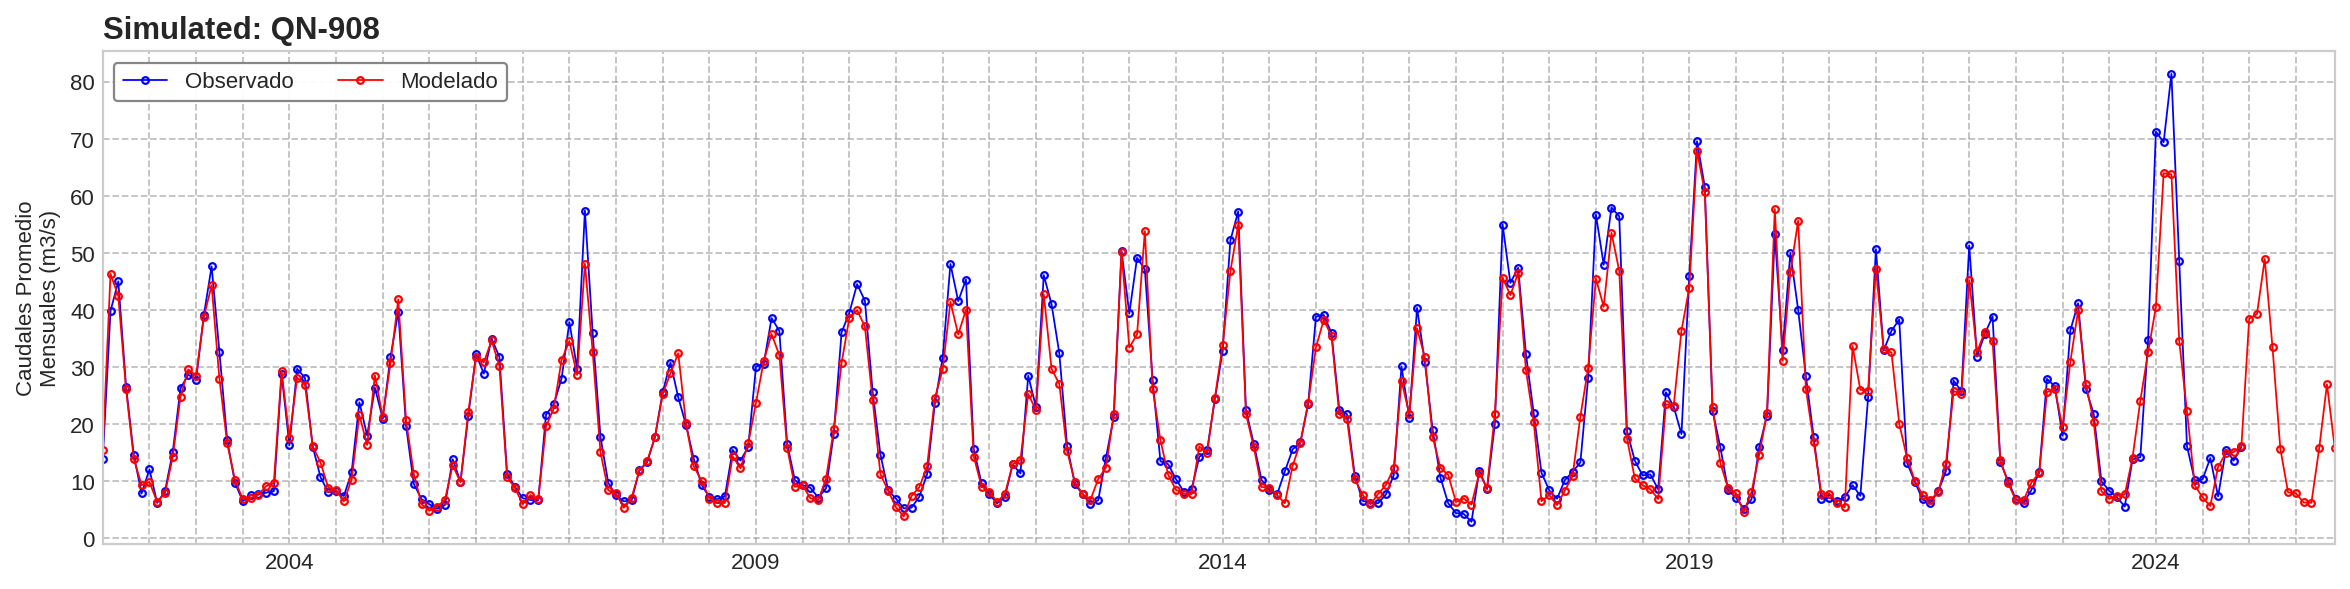
\includegraphics[width=1.\textwidth]{Figures/fig09a.png}
    \caption{Caudal Incremental Promedio Mensual (m3/s) en QN-908 Uchuhuerta (1998-2025)}
    \label{fig:9a1}
\end{figure}

\begin{table}[ht]
\centering
\caption{Indicadores estadísticos de desempeño del modelo VIC en QN-908 Uchuhuerta.}
\label{tab:swat_qn908}
\small
\begin{tabular}{lc}
\toprule
\textbf{Índice} & \textbf{Validación (2002–2025)} \\
\midrule
RMSE & 3.36 \\
PBIAS (\%) & -2.97 \\
RSR & 0.23 \\
NSE & 0.95 \\
Willmott d & 0.99 \\
r & 0.98 \\
R$^2$ & 0.95 \\
KGE & 0.91 \\
\bottomrule
\end{tabular}
\vspace{2pt}
\begin{minipage}{0.9\textwidth}
\small 
\textit{Nota.} RMSE: \textit{Root Mean Square Error}; PBIAS: \textit{Percent
Bias}; RSR: \textit{Ratio of the RMSE to the standard deviation of measured
data}; NSE: \textit{Nash-Sutcliffe Efficiency} \parencite{nash1970river}; r:
\textit{Coeficiente de correlación}; R$^2$: \textit{Coeficiente de
determinación}; d: \textit{Índice de Willmott}
\parencite{willmott1981validation}; KGE: \textit{Kling-Gupta Efficiency}
\parencite{gupta2009decomposition}.
\end{minipage}
\end{table}

La Figura \ref{fig:9a1} muestra los caudales promedio mensuales simulados y
observados en la estación QN-908 Uchuhuerta para el período comprendido entre
enero de 2002 y diciembre de 2025. Se aprecia que los picos de caudal alcanzan
valores cercanos a los 50~m\textsuperscript{3}/s, con máximos puntuales que
varían entre aproximadamente 60~m\textsuperscript{3}/s y
70~m\textsuperscript{3}/s (como en el año 2019). El caudal base se mantiene
relativamente constante alrededor de los 9~m\textsuperscript{3}/s a lo largo del
período. Durante el año 2025, los caudales simulan una variabilidad marcada, con
un máximo de 55.0~m\textsuperscript{3}/s en febrero y un mínimo de
9.6~m\textsuperscript{3}/s en mayo, según se observa en el gráfico.

\paragraph{6.2.2.2\quad QN-909 Huallamayo}\mbox{}\\
\addcontentsline{toc}{subsubsection}{6.2.2.2 \quad QN-909 Huallamayo}
La Figura \ref{fig:9b} presenta el hidrograma mensual promedio simulado por el
modelo VIC para la estación QN-909 Huallamayo, correspondiente al período
comprendido entre enero de 2002 y diciembre de 2025. Los resultados se comparan
con los caudales observados, permitiendo evaluar la capacidad del modelo para
reproducir la dinámica hidrológica mensual a lo largo de más de dos décadas.
Según el análisis estadístico mostrado en la Tabla \ref{tab:swat_qn909}, ambas
series presentan un buen nivel de concordancia, indicando que las simulaciones
reproducen adecuadamente el comportamiento hidrológico observado.

\begin{figure}[H]
    \centering
    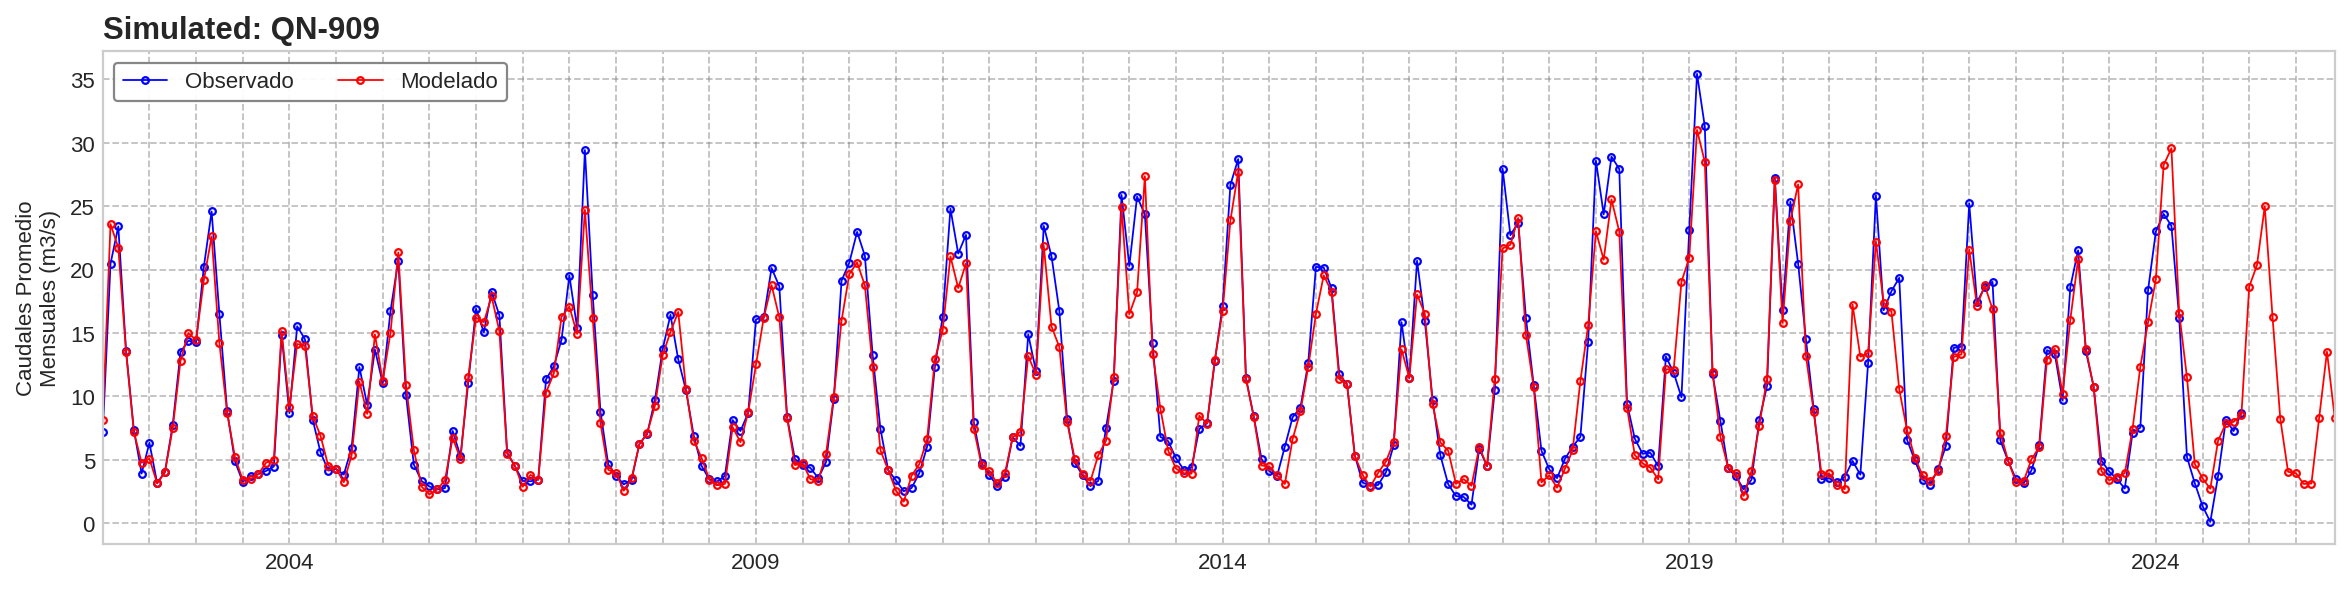
\includegraphics[width=1.\textwidth]{Figures/fig09b.png}
    \caption{Caudal Incremental Promedio Mensual (m\textsuperscript{3}/s) en
    QN-909 Huallamayo (2002–2025)}
    \label{fig:9b}
\end{figure}

\begin{table}[ht]
\centering
\caption{Indicadores estadísticos de desempeño del modelo VIC en QN-909 Huallamayo.}
\label{tab:swat_qn909}
\small
\begin{tabular}{lc}
\toprule
\textbf{Índice} & \textbf{Validación (2002–2025)} \\
\midrule
RMSE & 1.73 \\
PBIAS (\%) & -2.87 \\
RSR & 0.23 \\
NSE & 0.95 \\
Willmott d & 0.99 \\
r & 0.98 \\
R$^2$ & 0.95 \\
KGE & 0.90 \\
\bottomrule
\end{tabular}
\vspace{2pt}
\begin{minipage}{0.9\textwidth}
\small 
\textit{Nota.} RMSE: \textit{Root Mean Square Error}; PBIAS: \textit{Percent
Bias}; RSR: \textit{Ratio of the RMSE to the standard deviation of measured
data}; NSE: \textit{Nash-Sutcliffe Efficiency}; r: \textit{Coeficiente de
correlación}; R$^2$: \textit{Coeficiente de determinación}; d: \textit{Índice de
Willmott}; KGE: \textit{Kling-Gupta Efficiency}.
\end{minipage}
\end{table}

En general, el modelo logra captar satisfactoriamente la estacionalidad y
magnitud de los caudales observados, con un buen ajuste en la mayoría de los
picos y valles hidrológicos. Los caudales pico alcanzan valores del orden de los
35~m\textsuperscript{3}/s, especialmente durante los meses de avenida (entre
enero y marzo), mientras que el caudal base se mantiene en torno a los
4–6~m\textsuperscript{3}/s. Para el año 2025, se observan valores máximos
modelados de 27.5~m\textsuperscript{3}/s en febrero y mínimos cercanos a
4.8~m\textsuperscript{3}/s en junio.

\paragraph{6.2.2.3\quad QN-901 + QN-902 + QN-911}\mbox{}\\
\addcontentsline{toc}{subsubsection}{6.2.2.3 \quad QN-901 + QN-902 + QN-911}
La Figura \ref{fig:9c} presenta el hidrograma mensual promedio simulado por el
modelo VIC para el conjunto de estaciones QN-901, QN-902 y QN-911,
correspondiente al período comprendido entre enero de 2002 y diciembre de 2025.
Los resultados combinados permiten representar de forma integrada el
comportamiento hidrológico en esta sección de la cuenca. Según el análisis
estadístico mostrado en la Tabla \ref{tab:swat_qn901_qn911}, ambas series
presentan un buen nivel de concordancia, indicando que las simulaciones
reproducen adecuadamente el comportamiento hidrológico observado.

\begin{figure}[H]
    \centering
    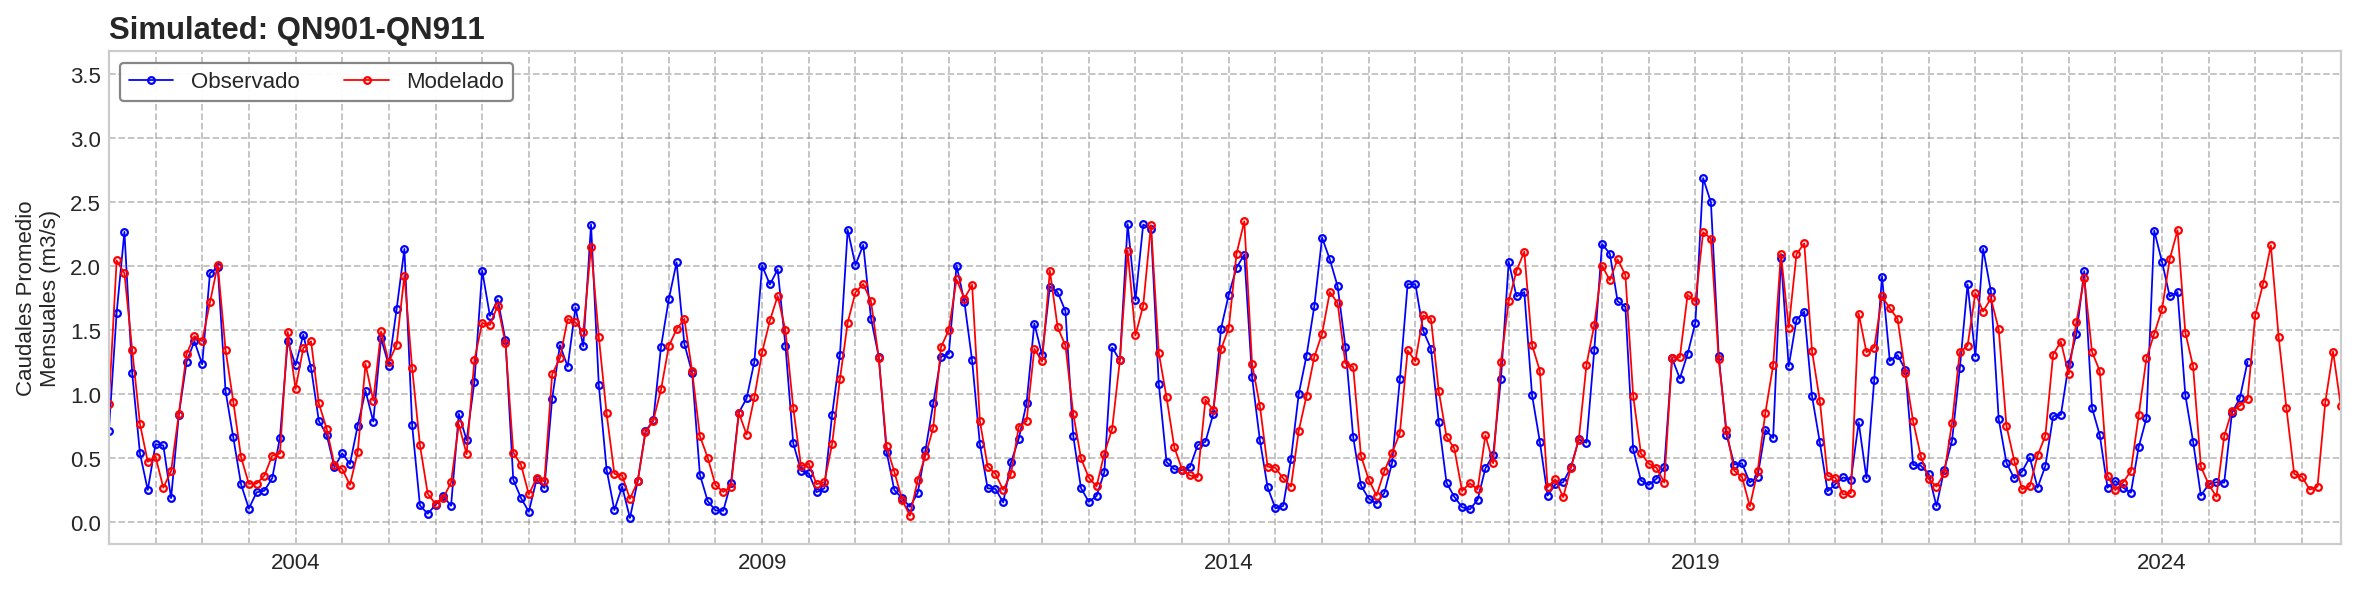
\includegraphics[width=1.\textwidth]{Figures/fig09c.png}
    \caption{Caudal Incremental Promedio Mensual (m\textsuperscript{3}/s) en
    QN-901 + QN-902 + QN-911 (2002–2025)}
    \label{fig:9c}
\end{figure}

\begin{table}[ht]
\centering
\caption{Indicadores estadísticos de desempeño del modelo VIC en QN-901, QN-902, QN-911 y el caudal agregado QN901-QN911.}
\label{tab:swat_qn901_qn911}
\small
\begin{tabular}{lcccc}
\toprule
\textbf{Índice} & \textbf{QN-901} & \textbf{QN-902} & \textbf{QN-911} &
\textbf{QN901-QN911} \\
\midrule
RMSE & 0.13 & 0.15 & 0.02 & 0.26 \\
PBIAS (\%) & 2.82 & 4.60 & 2.91 & 3.66 \\
RSR & 0.41 & 0.44 & 0.52 & 0.39 \\
NSE & 0.83 & 0.80 & 0.73 & 0.85 \\
Willmott d & 0.95 & 0.94 & 0.91 & 0.95 \\
r & 0.92 & 0.90 & 0.86 & 0.92 \\
R$^2$ & 0.84 & 0.81 & 0.73 & 0.85 \\
KGE & 0.82 & 0.82 & 0.73 & 0.84 \\
\bottomrule
\end{tabular}
\vspace{2pt}
\begin{minipage}{0.9\textwidth}
\small 
\textit{Nota.} RMSE: \textit{Root Mean Square Error}; PBIAS: \textit{Percent
Bias}; RSR: \textit{Ratio of the RMSE to the standard deviation of measured
data}; NSE: \textit{Nash-Sutcliffe Efficiency}; r: \textit{Coeficiente de
correlación}; R$^2$: \textit{Coeficiente de determinación}; d: \textit{Índice de
Willmott}; KGE: \textit{Kling-Gupta Efficiency}.
\end{minipage}
\end{table}

En la serie se observa una marcada estacionalidad, con picos de caudal que en
general no superan los 2.5~m\textsuperscript{3}/s y mínimos que pueden acercarse
a 0.3~m\textsuperscript{3}/s durante la temporada seca. Los caudales modelados
logran reproducir adecuadamente la dinámica hidrológica observada, con una buena
correspondencia en los patrones de ascenso y descenso estacional, aunque se
identifican algunas sobrestimaciones puntuales durante los períodos de crecida.
Durante el año 2025, los caudales simulados presentan un comportamiento
coherente con el patrón multianual, alcanzando un máximo de aproximadamente
2.2~m\textsuperscript{3}/s en febrero y un mínimo cercano a
0.4~m\textsuperscript{3}/s en julio.

\paragraph{6.2.2.4\quad QN-903 + QN-904 + QN-905}\mbox{}\\
\addcontentsline{toc}{subsubsection}{6.2.2.4 \quad QN-903 + QN-904 + QN-905}
La Figura \ref{fig:9d} presenta el hidrograma mensual promedio simulado por el
modelo VIC para el conjunto de estaciones QN-903, QN-904 y QN-905,
correspondiente al período comprendido entre enero de 2002 y diciembre de 2025.
Según el análisis estadístico mostrado en la Tabla \ref{tab:swat_qn903_qn905},
ambas series presentan un buen nivel de concordancia, indicando que las
simulaciones reproducen adecuadamente el comportamiento hidrológico observado.

\begin{figure}[H]
    \centering
    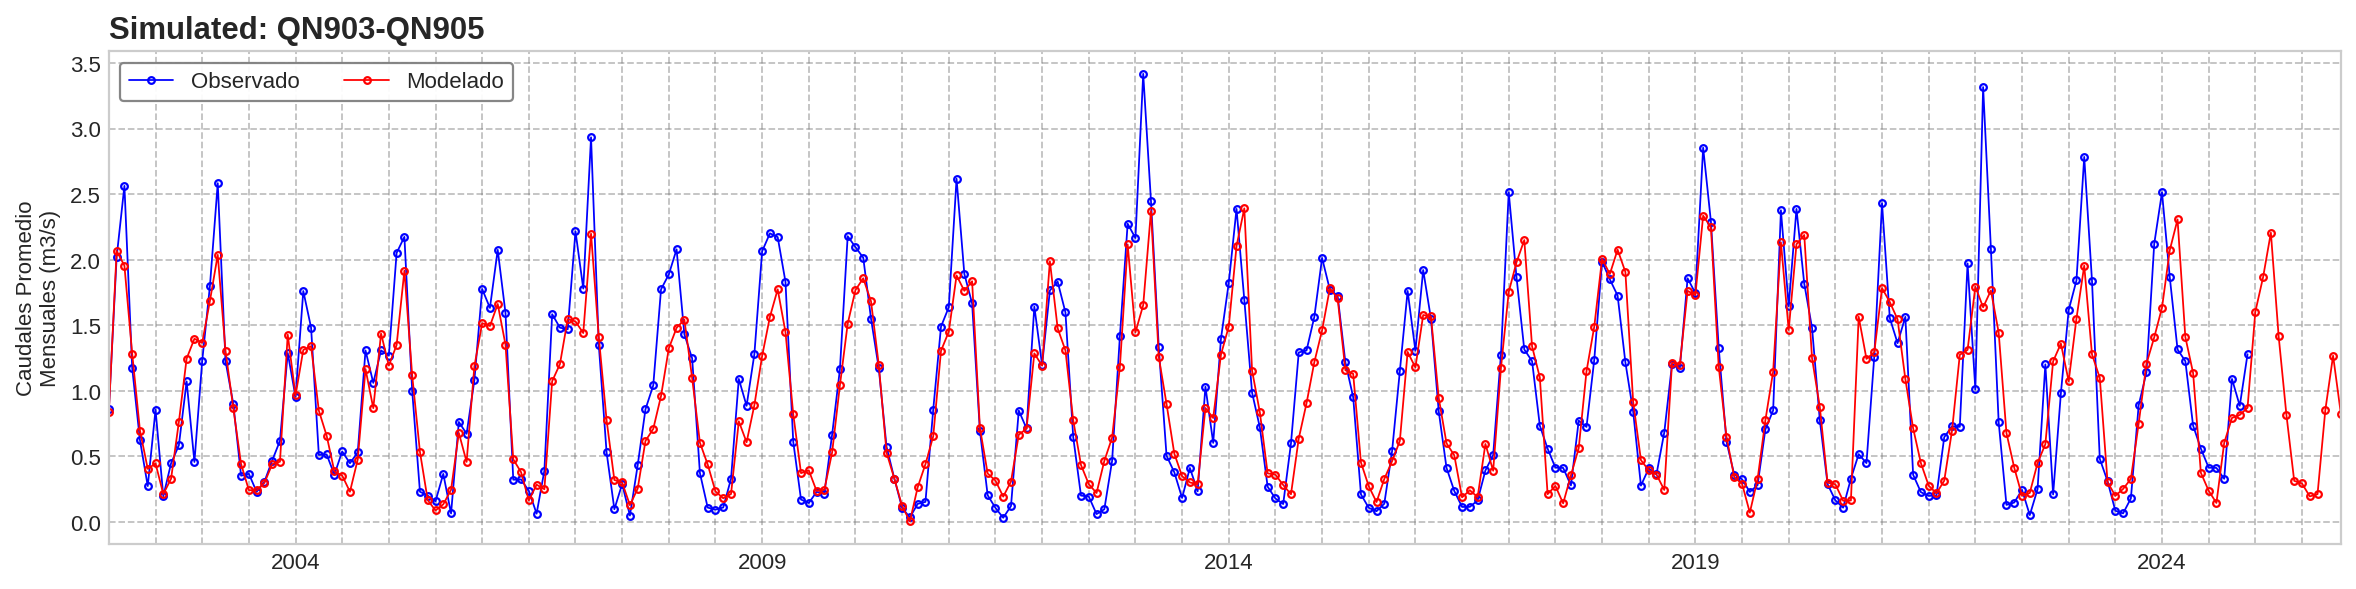
\includegraphics[width=1.\textwidth]{Figures/fig09d.png}
    \caption{Caudal Incremental Promedio Mensual (m\textsuperscript{3}/s) en
    QN-903 + QN-904 + QN-905 (2002–2025)}
    \label{fig:9d}
\end{figure}

\begin{table}[ht]
\centering
\caption{Indicadores estadísticos de desempeño del modelo VIC en QN-903, QN-904, QN-905 y el caudal agregado QN903-QN905.}
\label{tab:swat_qn903_qn905}
\small
\begin{tabular}{lcccc}
\toprule
\textbf{Índice} & \textbf{QN-903} & \textbf{QN-904} & \textbf{QN-905} &
\textbf{QN903-QN905} \\
\midrule
RMSE & 0.17 & 0.11 & 0.08 & 0.32 \\
PBIAS (\%) & -8.67 & -3.74 & -14.64 & -8.02 \\
RSR & 0.46 & 0.43 & 0.59 & 0.43\\
NSE & 0.79 & 0.81 & 0.65 & 0.81\\
Willmott d & 0.93 & 0.94 & 0.87 & 0.94 \\
r & 0.91 & 0.91 & 0.84 & 0.92 \\
R$^2$ & 0.82 & 0.82 & 0.71 & 0.84 \\
KGE & 0.75 & 0.79 & 0.61 & 0.76 \\
\bottomrule
\end{tabular}
\vspace{2pt}
\begin{minipage}{0.9\textwidth}
\small 
\textit{Nota.} RMSE: \textit{Root Mean Square Error}; PBIAS: \textit{Percent
Bias}; RSR: \textit{Ratio of the RMSE to the standard deviation of measured
data}; NSE: \textit{Nash-Sutcliffe Efficiency}; r: \textit{Coeficiente de
correlación}; R$^2$: \textit{Coeficiente de determinación}; d: \textit{Índice de
Willmott}; KGE: \textit{Kling-Gupta Efficiency}.
\end{minipage}
\end{table}

El modelo reproduce de manera adecuada la estacionalidad de los caudales
observados, con un buen ajuste en la mayoría de los máximos y mínimos mensuales.
Se aprecian picos de caudal de hasta 3.0~m\textsuperscript{3}/s en los meses de
avenida, mientras que los valores mínimos pueden llegar a estar por debajo de
0.3~m\textsuperscript{3}/s durante los meses secos. En el año 2025, los caudales
simulados presentan una dinámica coherente con el comportamiento multianual,
alcanzando un máximo de 2.3~m\textsuperscript{3}/s en febrero y un mínimo
cercano a 0.4~m\textsuperscript{3}/s en agosto.

\newpage
\section{DISCUSIONES Y CONCLUSIONES}

El presente estudio actualiza las series de caudales naturalizados del sistema
hídrico de la cuenca del río Paucartambo, utilizadas por la Central
Hidroeléctrica Yuncán de ENGIE Energía Perú S.A.A., en el marco de la
Resolución OSINERGMIN N° 196-2016-OS/CD y del Procedimiento Técnico N° 41. El
periodo de análisis comprende de 1965 a 2025, con énfasis en la simulación
hidrológica del intervalo 1998--2025.

La estimación de los caudales naturales se desarrolló mediante una metodología
de hidrología física distribuida basada en el modelo VIC (Variable Infiltration
Capacity). El modelo fue alimentado con precipitación CHIRPS, variables
meteorológicas de ERA5-Land e información geofísica de la cuenca. Las series de
precipitación fueron corregidas mediante \textit{quantile mapping}, y las
salidas de caudal del modelo incorporan un ajuste por desviación de sesgo antes
de su presentación.

Los caudales promedio mensuales se obtuvieron para los puntos de control QN-908
(Uchuhuerta), QN-909 (Huallamayo), QN-901 + QN-902 + QN-911 y QN-903 + QN-904 +
QN-905. Para estabilizar las condiciones internas del modelo, se consideró un
periodo de \textit{spin-up} de cuatro años antes del análisis de resultados.

El tiempo de desplazamiento estimado para el tramo Embalse Huallamayo--Casa de
Máquinas varía entre 0.64 y 6.4~h para los caudales representativos evaluados,
lo que permite caracterizar el retardo hidráulico asociado a la conducción desde
este punto de regulación.

La evaluación estadística indica una concordancia adecuada entre los caudales
simulados y observados en los puntos evaluados. Los indicadores NSE, RSR, PBIAS,
Willmott (d), coeficiente de correlación (r), coeficiente de determinación
(R$^2$) y KGE se presentan en las Tablas \ref{tab:swat_qn908} a
\ref{tab:swat_qn903_qn905}, y respaldan el uso de las series generadas para la
caracterización hidrológica mensual de la cuenca.

En conclusión, el estudio cumple con la actualización de las series de caudales
naturalizados para el periodo 1965--2025, incorporando información satelital,
reanálisis climático, modelación hidrológica distribuida y corrección por sesgo.
Los resultados constituyen una base técnica consistente para el análisis
hidrológico del sistema Yuncán y para futuras actualizaciones de la información
hidrometeorológica de la cuenca. Se recomienda mantener la actualización
periódica de los registros, mejorar la disponibilidad de observaciones en campo
y revisar los parámetros del modelo cuando se incorporen nuevas mediciones.

% \pagestyle{fancy}

% Bibliography (if needed)
% \printbibliography
\end{document}